\documentclass[11pt,a4paper]{article}

% ── Packages ────────────────────────────────────────────────────────────────
\usepackage[utf8]{inputenc}
\usepackage[T1]{fontenc}
\usepackage{amsmath,amssymb,amsfonts}
\usepackage{bm}
\usepackage{graphicx}
\usepackage{booktabs}
\usepackage[margin=2.5cm]{geometry}
\usepackage{hyperref}
\usepackage{cite}
\usepackage{xcolor}
\usepackage{enumitem}
\usepackage{cleveref}
\usepackage{subcaption}
\usepackage{float}
\usepackage{algorithm, algpseudocode}


% ── Title ────────────────────────────────────────────────────────────────────
\title{\textbf{Computing Periodic Orbits of the Lorenz System}\\[4pt]}
\author{Maximilian Hartenberger\\[2pt]}
\date{\today}

\begin{document}
\maketitle

\begin{abstract}
This report presents a computational pipeline for discovering unstable
periodic orbits of the Lorenz system at classical parameters
($\sigma=10$, $\rho=28$, $\beta=8/3$).  Candidate orbits are identified
as \emph{near-recurrences} --- close returns of a long numerically
integrated trajectory --- and then refined to machine precision via
L-BFGS minimisation of a multiple-shooting residual.  A full factorial
sweep over the number of shooting segments $N$ and the L-BFGS memory
depth $m$ ($7\times7$ grid, $\sim$29,000 independent cases) is deployed
on the Iridis~X HPC cluster using SLURM job arrays.  We find that
short-period orbits ($T \le 20$) converge with $>\!99\%$ success rate
using as few as $N=5$ segments --- demonstrating that near-recurrences
provide excellent initial guesses.  For longer periods the optimal $N$
scales with $T$ so that the per-segment integration time remains below
the Lyapunov time, and the maximal L-BFGS memory $m=320$ is
universally beneficial.  The best $(N,m)$ pair is tabulated for each
target period, giving practitioners a concrete starting point for
periodic-orbit searches in the Lorenz system and beyond.
\end{abstract}

% ============================================================================
\section{Introduction}
% ============================================================================

Periodic orbits are fundamental invariant sets of dynamical systems.  In
chaotic systems such as the Lorenz equations, unstable periodic orbits (UPOs)
form the \emph{skeleton} of the attractor: every trajectory on the strange
attractor can be viewed as wandering among the neighbourhoods of infinitely
many UPOs~\cite{cvitanovic2016chaos}.  Knowledge of these orbits is essential
for understanding the transport, statistics, and symbolic dynamics of the
system.

Computing UPOs numerically is challenging because they are unstable: a naive
forward integration will diverge exponentially from the orbit.  The standard
remedy is to formulate the problem as a root-finding equation and solve it
with a Newton-type method, using multiple shooting to manage the exponential
divergence over longer periods.  The convergence of such methods, however,
depends critically on the quality of the initial guess.

This project addresses the initial-guess problem by first scanning a long
trajectory for \emph{near-recurrences} --- pairs of times at which the flow
returns close to a previously visited state.  Each such near-recurrence
provides an approximate period $T_{\text{guess}}$ and a state vector
$u_{\text{rec}}$ that serve as the starting point for the refinement
stage.

% ============================================================================
\section{The Lorenz System}
% ============================================================================

The Lorenz system~\cite{lorenz1963deterministic} is the three-dimensional
system of ordinary differential equations
\begin{equation}\label{eq:lorenz}
\begin{aligned}
  \dot{x} &= \sigma\,(y - x), \\
  \dot{y} &= x\,(\rho - z) - y, \\
  \dot{z} &= x\,y - \beta\,z,
\end{aligned}
\end{equation}
with the classical parameter values $\sigma = 10$, $\rho = 28$,
$\beta = 8/3$.  At these values the system exhibits a chaotic strange
attractor --- the iconic ``Lorenz butterfly.''

Let $u(t) = (x(t), y(t), z(t)) \in \mathbb{R}^3$ denote
the state at time $t$.  The right-hand side of~\eqref{eq:lorenz} defines a
vector field $f: \mathbb{R}^3 \to \mathbb{R}^3$, so that
\begin{equation}
  \dot{u}(t) = f\bigl(u(t)\bigr).
\end{equation}
The \emph{flow} $\varphi: \mathbb{R} \times \mathbb{R}^3 \to \mathbb{R}^3$ advances an
initial condition $u_0$ forward by time $t$:
\begin{equation}
  \varphi(t, u_0) = u(t),
  \qquad \dot{u} = f(u), \quad u(0) = u_0.
\end{equation}
All numerical integrations in this work use the classic fourth-order
Runge--Kutta scheme (RK4) with a fixed time step $\Delta t = 0.01$.
The Lorenz right-hand side and the RK4 integrator are provided by the
Julia package \texttt{ToySystems.jl}
(\url{https://github.com/Davide-Lasagna-s-Lab/ToySystems.jl}),
which exposes the Lorenz equations in both nonlinear and linearised forms.

% ============================================================================
\section{Mathematical Preliminaries}
% ============================================================================

Before formulating the periodic-orbit problem, we establish the mathematical
objects on which the computation rests: the nonlinear flow, its linearisation,
and the adjoint flow.  All three are provided \textbf{matrix-free} by the
Julia packages \texttt{Flows.jl} and \texttt{NKSearch.jl}; no Jacobian matrix
is ever assembled.

\subsection{Nonlinear Flow}
Let $f \in C^k(\mathbb{R}^n)$ denote the right-hand side of a dynamical
system ($n = 3$ for Lorenz).  The \emph{flow map}
$\varphi: \mathbb{R} \times \mathbb{R}^n \to \mathbb{R}^n$ advances an
initial condition $u_0$ forward by time $t$:
\begin{equation}\label{eq:flow_def}
  \varphi(t, u_0) = u(t),
  \qquad \dot{u} = f(u), \quad u(0) = u_0.
\end{equation}
It satisfies $\frac{\partial \varphi}{\partial t}(t, u_0)
= f(\varphi(t, u_0))$.  In this work $\varphi$ is discretised with the
classical fourth-order Runge--Kutta scheme (RK4) at fixed step $\Delta t$.

\subsection{Linearised Flow}
Differentiating the flow with respect to the initial condition yields the
\emph{linearised flow} (or state-transition matrix)
$\Phi(t, u_0) := \frac{\partial \varphi}{\partial u_0}(t, u_0)$.  Swapping
the order of differentiation and applying the chain rule gives the variational
equation
\begin{equation}\label{eq:lin_flow}
  \frac{\partial \Phi}{\partial t} = Df(\varphi(t, u_0))\,\Phi(t, u_0),
  \qquad \Phi(0, u_0) = I.
\end{equation}
For an initial perturbation $v_0$, the variation
$v(t) := \Phi(t, u_0)\,v_0$ satisfies
\begin{equation}\label{eq:lin_var}
  \dot{v} = Df(\varphi(t, u_0))\,v, \qquad v(0) = v_0.
\end{equation}
For better understanding, we can look at the linearized flow as a linear approximation of the flow $\varphi$ in the following way: Let $v_0=u_0-\bar{u}_0$ be a small perturbation of the initial condition $\bar{u}_0$. Then using Taylor expansion we have
\begin{equation*}
    \varphi(t,\bar{u}_0) = \varphi(t,u_0) - \Phi(t,u_0)v_0 + \mathcal{O}(\|v_0\|^2).
\end{equation*}
The linearized flow $\Phi$ is the first order approximation of the flow $\varphi$ with respect to the initial condition.
\begin{align*}
    \Phi(t,u_0)(u_0-\bar{u}_0) &= \varphi(t,u_0) - \varphi(t,\bar{u}_0) + \mathcal{O}(\|u_0-\bar{u}_0\|^2)\\
    &\approx \varphi(t,u_0) - \varphi(t,\bar{u}_0).
\end{align*}

\subsection{Adjoint Flow}
The \emph{adjoint flow} $\Psi(t, u_0) := \Phi(t, u_0)^\top$ maps a final
variation backward to the initial variation.  Let $q_T$ be a final variation
at time $T$.  Then
\begin{equation*}
    \Psi(T, u_0)\,q_T = q(0).
\end{equation*}
Define $q(t) := \Psi(T - t, \varphi(t, u_0))\,q_T$.
Using the cocycle property of the linearised flow
$\Phi(t+s, u_0) = \Phi(t, \varphi(s, u_0))\,\Phi(s, u_0)$,
we have
\begin{equation*}
    \Phi(T, u_0) = \Phi(T - t, \varphi(t, u_0))\,\Phi(t, u_0).
\end{equation*}
Taking the transpose gives the adjoint cocycle property
$\Psi(T, u_0) = \Psi(t, u_0)\,\Psi(T - t, \varphi(t, u_0))$.
Consequently
\begin{align*}
    q(0) &= \Psi(T, u_0)\,q_T \\
         &= \Psi(t, u_0)\,\Psi(T - t, \varphi(t, u_0))\,q_T \\
         &= \Psi(t, u_0)\,q(t),
\end{align*}
and thus $q(t) = \Psi(t, u_0)^{-1}q(0) = \Phi(t, u_0)^{-\top}q(0)$.
Differentiating with respect to $t$ and using
$\frac{d}{dt}M^{-1} = -M^{-1}\dot{M}M^{-1}$ gives
\begin{align*}
    \frac{\partial q}{\partial t}
    &= -\Phi(t, u_0)^{-\top}
       \frac{\partial \Phi}{\partial t}(t, u_0)^{\top}
       \Phi(t, u_0)^{-\top} q(0) \\
    &= -\Phi(t, u_0)^{-\top}
       \bigl(Df(\varphi(t, u_0))\,\Phi(t, u_0)\bigr)^{\top}
       \Phi(t, u_0)^{-\top} q(0) \\
    &= -Df(\varphi(t, u_0))^{\top}\,q(t).
\end{align*}
Thus the adjoint variation $q$ satisfies the backward-in-time ODE
\begin{equation}\label{eq:adjoint_flow}
  \dot{q} = -Df(\varphi(t, u_0))^\top\,q, \qquad q(T) = q_T.
\end{equation}
A key duality relation holds: for any forward variation
$v(t) = \Phi(t, u_0) v_0$ and adjoint variation $q(t)$,
\begin{equation}\label{eq:duality}
  \langle q_T, v(T) \rangle
  = \langle q_T, \Phi(T, u_0) v_0 \rangle
  = \langle \Phi(T, u_0)^\top q_T, v_0 \rangle
  = \langle \Psi(T, u_0) q_T, v_0 \rangle
  = \langle q(0), v_0 \rangle.
\end{equation}
That is, the scalar product of forward and adjoint variations is conserved
in time.

\subsection{Matrix-Free Implementation in NKSearch.jl}\label{sec:prelim_impl}
All three flows --- nonlinear $\varphi$, linearised $\Phi$, and adjoint
$\Psi$ --- act \textbf{matrix-free}: only the action of $Df$ on a vector is
computed, never the full Jacobian.  The RK4 integrator stores its four
internal stages ($k_1, \dots, k_4$) in a \texttt{RAMStageCache} during the
nonlinear propagation.  The linearised and adjoint flows read these
\textbf{same} cached stages via \texttt{TimeStepFromCache}, evaluating
$Df(x_{\text{stage}, i}) \cdot v$ at the stored base states.  Because
forward and adjoint propagators share the identical stage cache,
\begin{equation}
  \langle \Phi_h \cdot v_0,\; q_T \rangle
  = \langle v_0,\; \Psi_h \cdot q_T \rangle
\end{equation}
holds to machine precision --- the discrete transpose relationship is exact.

Internally, \texttt{NKSearch.jl} deep-copies each flow once per shooting
segment for thread safety and constructs two caches:
\begin{itemize}
  \item \textbf{Forward cache} (\texttt{StageIterCache}): stores the
        nonlinear and linearised flows, manages the stage caches, and
        evaluates the residual $F(z)$ via \texttt{update!}.
  \item \textbf{Adjoint cache} (\texttt{AdjointIterSolCache}): stores the
        adjoint flows and shares the stage caches, end-of-segment states,
        and time derivatives with the forward cache, computing
        $J^\top \cdot F(z)$ via \texttt{mul!}.
\end{itemize}
This architecture is the computational engine behind the L-BFGS gradient
evaluation described in section \ref{sec:lbfgs}.

% ============================================================================
\section{Periodic Orbits: Definition and Problem Statement}
% ============================================================================

A \emph{periodic orbit} of period $T > 0$ is a solution
$u(t)$ of~\eqref{eq:lorenz} satisfying
\begin{equation}\label{eq:periodic}
  u(t + T) = u(t) \qquad \forall\, t \in \mathbb{R}.
\end{equation}
Equivalently, a point $u_0$ lies on a periodic orbit of period $T$
if and only if
\begin{equation}\label{eq:periodic_condition}
  \varphi(T, u_0) = u_0.
\end{equation}

Condition~\eqref{eq:periodic_condition} can be expressed as the root-finding
problem
\begin{equation}\label{eq:root}
  \tilde{F}(u_0, T) \;\equiv\; \varphi(T, u_0) - u_0
  \;=\; 0.
\end{equation}
Equation~\eqref{eq:root} is under-determined: there are four unknowns
($u_0 \in \mathbb{R}^3$ and $T \in \mathbb{R}$) but only three
equations.  This reflects the fact that every point on a given periodic orbit
is a valid $u_0$ for the same $T$.  The standard resolution is to
add a \emph{phase condition} that selects a unique point on the orbit, for
instance
\begin{equation}
  \bigl\langle f(u_0),\; u_0 - u_{\text{ref}} \bigr\rangle = 0,
\end{equation}
which pins $u_0$ to a Poincar\'{e} section orthogonal to the flow
and passing through a reference state $u_{\text{ref}}$.

For long periods $T$, the single-shooting formulation~\eqref{eq:root} suffers
from extreme sensitivity to the initial condition because the Lorenz system
is chaotic: a perturbation $\delta u_0$ grows as
$\|\delta u(T)\| \sim e^{\lambda T} \|\delta u_0\|$, where
$\lambda > 0$ is the largest Lyapunov exponent.  This makes the root-finding
problem ill-conditioned.  The standard cure is \emph{multiple shooting}, which we describe in section \ref{sec:multiple_shooting}.

% ============================================================================
\section{Near-Recurrences: Concept and Mathematical Definition}
% ============================================================================

\subsection{Intuition}
On a chaotic attractor, a long trajectory $\{u(t)\}_{t \ge 0}$ will,
by the Poincar\'{e} recurrence theorem, eventually return arbitrarily close
to any previously visited state.  In practice, for a finite-time simulation,
the trajectory will exhibit many \emph{near-returns} --- pairs of times
$t_i < t_j$ for which the states are close in phase space:
\begin{equation}
  \|u(t_j) - u(t_i)\| \ll 1.
\end{equation}
If the distance is small enough, the segment of trajectory between $t_i$ and
$t_j$ is a good approximation to a periodic orbit, and
$T_{\text{guess}} \approx t_j - t_i$ is a good estimate of its period.

\subsection{Formal Definition}
Let $u^{(0)}, u^{(1)}, u^{(2)}, \dots$ be a
discrete trajectory sampled every $\Delta t$ from a long forward integration
starting from $u^{(0)} = (1,1,1)^{\mathsf{T}}$.  That is,
\begin{equation}
  u^{(k)} = \varphi^{k\Delta t}(u^{(0)}), \qquad k = 0, 1, 2, \dots
\end{equation}

A \emph{near-recurrence} at discrete-time shift $s$ is a pair of indices
$(k, k+s)$ such that the Euclidean distance between the two states falls
below a threshold $\varepsilon$:
\begin{equation}\label{eq:near_recurrence}
  d(k, s) \;\equiv\; \bigl\|u^{(k+s)} - u^{(k)}\bigr\|
  \;<\; \varepsilon.
\end{equation}
The approximate period associated with this recurrence is
\begin{equation}
  T_{\text{guess}} = s \cdot \Delta t,
\end{equation}
and the recurrence state is $u_{\text{rec}} = u^{(k)}$ (or,
equivalently, any $u^{(k)}$ along the approximately closed loop).

In words: if the flow returns to within a distance $\varepsilon$ of a
previously visited point after $s$ time steps, we have found a candidate for
a periodic orbit of approximate period $s\Delta t$.

\subsection{Why This Works for the Lorenz Attractor}
The Lorenz attractor has a densely woven structure: unstable periodic orbits
of many different periods coexist and organise the flow.  When a trajectory
comes within a small distance of itself after some time $s\Delta t$, it is
typically shadowing an actual UPO of period close to $s\Delta t$.  The
near-recurrence provides an initial condition $u_{\text{rec}}$ that
lies within the basin of convergence of Newton's method for that UPO.  The
closer the recurrence (smaller $d$), the more likely the subsequent
optimisation will converge.

% ============================================================================
\section{Finding Near-Recurrences: Algorithm}
% ============================================================================

\subsection{Overview of the Pipeline}
The recurrence-detection stage is implemented in the Julia script
\texttt{scripts/find\_recurrences.jl}.  For each target period
$T_{\text{target}} \in \{5, 10, 20, 40, 80, 160\}$, the script:
\begin{enumerate}[label=(\roman*)]
  \item Generates a long reference trajectory by integrating the Lorenz
        equations with RK4 from $u^{(0)} = (1,1,1)^{\mathsf{T}}$,
        with step $\Delta t = 0.01$;
  \item Searches a narrow window of time shifts around
        $T_{\text{target}} / \Delta t$ for all pairs of states within
        distance $\varepsilon = 0.5$;
  \item Filters candidates to those whose approximate period lies within
        $\pm 20\%$ of $T_{\text{target}}$;
  \item Greedy-deduplicates the candidates by spatial separation, keeping
        only recurrences whose state vectors are pairwise separated by at
        least $\delta_{\min} = 3.0$ in phase space.
\end{enumerate}

\subsection{Search Window and Streaming Distance Matrix}
For a given target period $T_{\text{target}}$, we expect near-recurrences at
time shifts $s \approx T_{\text{target}} / \Delta t$.  Rather than computing
the full $O(K^2)$ distance matrix for a trajectory of length $K$, we use a
\emph{streaming distance matrix} that only compares each state with a
restricted range of future states:
\begin{equation}
  s \in \bigl[s_{\text{centre}} - w,\; s_{\text{centre}} + w\bigr],
  \qquad s_{\text{centre}} = \operatorname{round}\!\left(\frac{T_{\text{target}}}{\Delta t}\right),
\end{equation}
where the search half-width is $w = 200$ steps (corresponding to a period
range of $\pm 2.0$ time units around $T_{\text{target}}$).  The streaming
implementation, provided by the Julia package\\
\texttt{StreamingRecurrenceAnalysis.jl}\\
(\url{https://github.com/Davide-Lasagna-s-Lab/StreamingRecurrenceAnalysis.jl}),
processes the trajectory in a single
pass and collects all pairs $(i, j)$ whose distance falls below the threshold
$\varepsilon$:
\begin{equation}\label{eq:streaming}
  \mathcal{R}_{\text{raw}}
  = \bigl\{ (k, s) \;\big|\;
           d(k, s) < \varepsilon,\;
           s \in [s_{\text{centre}} - w,\; s_{\text{centre}} + w]
    \bigr\}.
\end{equation}
The maximum number of ``views'' (distance computations) is set to
$n_{\text{views}} = 900,\!000$, which limits the total computational cost of
the scan.

\subsection{Period Filtering}
From the raw set $\mathcal{R}_{\text{raw}}$, we retain only those
recurrences whose approximate period $T_{\text{guess}} = s\Delta t$ is within
a specified tolerance of the target:
\begin{equation}\label{eq:period_filter}
  \frac{|T_{\text{guess}} - T_{\text{target}}|}{T_{\text{target}}}
  \;\le\; \tau,
  \qquad \tau = 0.20.
\end{equation}
This ensures that the candidate is a plausible initial guess for a periodic
orbit of the desired period, rather than a harmonic or a near-recurrence at
an unrelated time scale.

\subsection{Greedy Spatial Deduplication}
The remaining candidates may cluster around the same underlying periodic
orbit: a single UPO can produce many near-recurrences at slightly different
phases or with minor variations in approximate period.  To avoid redundant
computation in the optimisation stage, we apply a greedy deduplication:

\begin{enumerate}[label=(\roman*)]
  \item Sort the filtered recurrences by ascending distance $d$ (closest
        recurrences are the most promising candidates);
  \item Iterate through the sorted list; for each candidate, accept it only
        if its state vector $u$ is at distance at least
        $\delta_{\min}$ from every \emph{already accepted} candidate:
        \begin{equation}\label{eq:dedup}
          \forall\,u_{\text{kept}} \in \mathcal{K},\qquad
          \|u - u_{\text{kept}}\| \;\ge\; \delta_{\min}.
        \end{equation}
\end{enumerate}
The threshold $\delta_{\min} = 3.0$ is chosen empirically; it is large enough
to distinguish genuinely distinct orbits on the Lorenz attractor
(characteristic size $\sim\!40$) while small enough not to discard valid
distinct candidates.

This procedure yields a set $\mathcal{K}$ of \emph{distinct near-recurrence
candidates}, each characterised by:
\begin{itemize}
  \item A state vector $u_{\text{rec}} \in \mathbb{R}^3$,
  \item An approximate period $T_{\text{guess}}$,
  \item A discrete-time shift $s$,
  \item A recurrence distance $d = \|u^{(k+s)} - u^{(k)}\|$.
\end{itemize}

\subsection{Output}
The deduplicated candidates are saved to CSV files, one per target period,
under \texttt{recurrences/TXX/recurrences.csv}.  Each file contains up to 100
candidates (ranked by recurrence distance, closest first), with the columns:
\texttt{rec\_id}, \texttt{u1}, \texttt{u2}, \texttt{u3}, \texttt{T\_guess},
\texttt{shift}, \texttt{distance}.

% ============================================================================
\section{Summary of Key Parameters}
% ============================================================================

\begin{table}[htbp]
  \centering
  \caption{Parameters used in the near-recurrence detection stage.}
  \label{tab:parameters}
  \begin{tabular}{@{}lll@{}}
    \toprule
    \textbf{Symbol} & \textbf{Value} & \textbf{Description} \\
    \midrule
    $\Delta t$          & $0.01$           & RK4 integration step \\
    $T_{\text{target}}$ & $\{5,10,20,40,80,160\}$ & Target orbit periods \\
    $\varepsilon$       & $0.5$            & Maximum recurrence distance (Eq.~\ref{eq:near_recurrence}) \\
    $w$                 & $200$ steps      & Search half-window around $s_{\text{centre}}$ \\
    $\tau$              & $0.20$           & Period tolerance (Eq.~\ref{eq:period_filter}) \\
    $\delta_{\min}$     & $3.0$            & Minimum spatial separation for distinctness (Eq.~\ref{eq:dedup}) \\
    $n_{\text{views}}$  & $900,\!000$      & Maximum distance computations in streaming scan \\
    \bottomrule
  \end{tabular}
\end{table}

% ============================================================================
\section{Multiple Shooting for Periodic Orbits}\label{sec:multiple_shooting}
% ============================================================================

\subsection{Motivation}
The single-shooting condition $\varphi(T, u_0) = u_0$
(Eq.~\ref{eq:periodic_condition}) is ill-conditioned for chaotic systems: an
initial perturbation $\delta u_0$ grows as
$\|\delta u(T)\| \sim e^{\lambda T}\|\delta u_0\|$, where
$\lambda > 0$ is the leading Lyapunov exponent of the Lorenz attractor
($\lambda \approx 0.91$).  For $T = 80$, this amplifies errors by a factor
of $\sim\!10^{31}$, rendering the Jacobian numerically singular and the
root-finding problem intractable.

\emph{Multiple shooting}~\cite{sanchez2004newton} circumvents this by
splitting the orbit into $N$ shorter segments, each integrated only over time
$T/N$.  The exponential amplification per segment is reduced to
$e^{\lambda T / N}$, which can be kept $O(1)$ by choosing $N$ sufficiently
large.

\subsection{Formulation}
Partition the period-$T$ orbit into $N$ segments of equal duration $T/N$.
Let $u_i \in \mathbb{R}^3$ be the state at the beginning of segment
$i$ ($i = 1, \dots, N$).  The segment is integrated forward:
\begin{equation}\label{eq:segment_integration}
  \varphi(T/N, u_i) = u_{i+1},
  \qquad i = 1, \dots, N,
\end{equation}
with the periodic wrap-around convention $u_{N+1} \equiv u_1$.

The unknown vector collects all shooting points and the period:
\begin{equation}
    z = \begin{pmatrix} u_1 \\ \vdots \\ u_N \\ T \end{pmatrix}
\end{equation}

The \emph{continuity constraints} require that the end of each segment
matches the beginning of the next.  This defines the \textbf{unaugmented
residual} $\tilde{F}: \mathbb{R}^{3N+1} \to \mathbb{R}^{3N}$:
\begin{equation}\label{eq:full_residual}
  \tilde{F}(z) =
  \begin{pmatrix}
    \varphi(T/N, u_1) - u_2 \\
    \varphi(T/N, u_2) - u_3 \\
    \vdots \\
    \varphi(T/N, u_N) - u_1
  \end{pmatrix}.
\end{equation}

\subsection{Jacobian of the Residual}
The Jacobian $D\tilde{F}(z) \in \mathbb{R}^{3N \times (3N+1)}$ has a
block-bidiagonal structure inherited from the segment coupling.  Let
$\Phi_i := \Phi(T/N, u_i)$ denote the linearised flow (state-transition
matrix) along segment $i$, and let
$f_i := f(\varphi(T/N, u_i))$ be the velocity at the end of the segment.
Then
\begin{equation}\label{eq:jacobian}
  D\tilde{F}(z) =
  \begin{pmatrix}
    \Phi_1 & -I & 0      & \dots  & 0      & \frac{1}{N}f_1 \\[4pt]
    0      & \Phi_2 & -I & \dots  & 0      & \frac{1}{N}f_2 \\[4pt]
    \vdots & \vdots & \vdots & \ddots & \vdots & \vdots \\[4pt]
    -I     & 0      & 0      & \dots  & \Phi_N & \frac{1}{N}f_N
  \end{pmatrix}.
\end{equation}
The last column arises from differentiating $\varphi(T/N, u_i)$ with respect
to $T$: $\frac{\partial}{\partial T}\varphi(T/N, u_i)
= \frac{1}{N}f(\varphi(T/N, u_i))$.  Each block is $3 \times 3$; the full
matrix has $3N$ rows and $3N+1$ columns --- it is one column short of being
square, reflecting the time-translation symmetry of periodic orbits.

\subsection{Phase Condition}
The system $\tilde{F}(z) = 0$ is under-determined ($3N$ equations for $3N+1$
unknowns).  If $\{u_i\}_{i=1}^N$ is a solution, shifting each point along the
orbit by the same time offset yields another valid solution.  We fix this
gauge freedom by requiring that the first shooting point lies in a
Poincar\'{e} section orthogonal to the local velocity:
\begin{equation}\label{eq:phase_condition}
  \langle u_1 - u_{\text{ref}},\; f(u_{\text{ref}}) \rangle = 0,
\end{equation}
where $u_{\text{ref}}$ is a reference point.  We take
$u_{\text{ref}} = u_{\text{rec}}$, the recurrence state, so that the phase
condition is automatically satisfied at the initial guess:
$\langle u_{\text{rec}} - u_{\text{rec}},\, f(u_{\text{rec}}) \rangle = 0$.
Appending this scalar equation to the residual and its
gradient row to the Jacobian gives the \textbf{augmented} system
$F: \mathbb{R}^{3N+1} \to \mathbb{R}^{3N+1}$:
\begin{equation}\label{eq:augmented_residual}
  F(z) =
  \begin{pmatrix}
    \varphi(T/N, u_1) - u_2 \\
    \vdots \\
    \varphi(T/N, u_N) - u_1 \\
    0
  \end{pmatrix},
  \qquad
  J(z) := DF(z) =
  \begin{pmatrix}
    \Phi_1 & -I & 0      & \dots  & 0      & \frac{1}{N}f_1 \\[4pt]
    0      & \Phi_2 & -I & \dots  & 0      & \frac{1}{N}f_2 \\[4pt]
    \vdots & \vdots & \vdots & \ddots & \vdots & \vdots \\[4pt]
    -I     & 0      & 0      & \dots  & \Phi_N & \frac{1}{N}f_N \\[4pt]
    f(u_{\text{ref}})^\top & 0 & 0 & \dots & 0 & 0
  \end{pmatrix}.
\end{equation}
The phase-condition row $f(u_{\text{ref}})^\top$ is constant (independent of
$z$) because we fix the reference at the start of the optimisation.  The zero
appended to $\tilde{F}$ ensures matching dimensions; the phase condition is
identically satisfied at the initial guess by construction, so its residual
entry remains zero throughout.

\subsection{Least-Squares Reformulation}
Rather than solving $F(z) = 0$ directly with Newton's method (which requires
$J(z)$ to be well-conditioned and involves solving a $(3N+1) \times (3N+1)$
linear system at each iteration), we minimise the scalar cost function
\begin{equation}\label{eq:cost}
  \phi(z) = \frac{1}{2}\bigl\|F(z)\bigr\|^2,
\end{equation}
whose global minimum $\phi = 0$ corresponds to an exact periodic orbit.  The
gradient of $\phi$ is
\begin{equation}\label{eq:gradient}
  \nabla\phi(z) = J(z)^{\top}\,F(z),
\end{equation}
which can be computed matrix-free using the adjoint flow (section \ref{sec:adjoint_impl}).
This least-squares formulation is the starting point for the L-BFGS
optimisation described in the next section.

% ============================================================================
\section{L-BFGS Optimisation}\label{sec:lbfgs}
% ============================================================================

\subsection{The L-BFGS Method}
The Limited-memory Broyden--Fletcher--Goldfarb--Shanno (L-BFGS) method
~\cite{nocedal2006numerical,liu1989limited} is a quasi-Newton algorithm for
minimising $\phi(z) = \frac{1}{2}\|F(z)\|^2$.  The true Hessian of $\phi$
is
\begin{equation}\label{eq:hessian}
  \nabla^2\phi(z) = J(z)^\top J(z)
  + \sum_{i=1}^{3N+1} F_i(z)\,\nabla^2 F_i(z),
\end{equation}
where $J(z) = DF(z)$ is the augmented Jacobian (Eq.~\ref{eq:augmented_residual}).
Near a solution ($F_i \approx 0$), the second term is negligible and
$\nabla^2\phi \approx J^\top J$, the Gauss--Newton approximation.
L-BFGS builds an approximation
$H_k \approx \bigl(\nabla^2 \phi(z_k)\bigr)^{-1}$
to the inverse Hessian using only the past $m$ gradient differences
$s_j = z_{j+1} - z_j$ and
$y_j = \nabla\phi(z_{j+1}) - \nabla\phi(z_j)$.
At each iteration $k$, the search direction is computed via the \textbf{two-loop
recursion} (Algorithm~\ref{alg:two_loop}):
\begin{equation}\label{eq:lbfgs_direction}
  d_k = -H_k\,\nabla\phi(z_k),
\end{equation}
and a backtracking line search determines the step length
$\lambda$ satisfying the simple decrease condition
$\phi(z_k + \lambda d_k) < \phi(z_k)$.  The state is then updated:
$z_{k+1} = z_k + \lambda d_k$.

The gradient $\nabla\phi(z) = J(z)^\top F(z)$ is evaluated
\textbf{matrix-free} using the discrete adjoint (see \S\ref{sec:adjoint_impl}).
The key advantage of L-BFGS for this problem is that it requires only
gradient information --- not the full Hessian --- and the
limited-memory form stores only $O(m)$ vectors rather than an
$O((3N+1)^2)$ matrix.  This is essential when $N$ is large (up to 320
segments, giving 961 unknowns).  The memory parameter $m$ controls how
many past curvature pairs are retained; larger $m$ gives a richer Hessian
approximation at the cost of greater storage.

\textbf{Implementation in NKSearch.jl.}
The L-BFGS method is implemented in \texttt{NKSearch.jl/src/search\_lbfgs.jl}.
The main function \texttt{\_search\_lbfgs\_opt!} receives both the forward
cache \texttt{fwd\_cache} (\texttt{StageIterCache}) and the adjoint cache
\texttt{adj\_cache} (\texttt{AdjointIterSolCache}), pre-built by the dispatch
layer.  The two caches share stage caches, end-of-segment states, and time
derivatives; \texttt{update!} populates them, and the adjoint \texttt{mul!}
reads them to compute $J^\top \cdot F(z)$.  The state is stored in an
\texttt{OptLBFGSCache} struct containing circular buffers
\texttt{s\_history, y\_history} of \texttt{MVector}s for the step--gradient
pairs, the current residual and gradient, the previous iterate, the effective
history length $n_{\text{hist}}$ (capped at $m$), and the search direction.
The line search (\texttt{linesearch\_opt\_lbfgs}) backtracks from $\lambda=1$,
reducing $\lambda$ by $\rho=0.5$ at each rejection; invalid evaluation points
(from integration failures) are caught via try--catch and treated as failures.

\begin{algorithm}[H]
\caption{L-BFGS for $\min_z \frac{1}{2}\|F(z)\|^2$}
\label{alg:lbfgs}
\begin{algorithmic}[1]
\State \textbf{Input:} initial guess $z_0$, memory size $m$, tolerances $\varepsilon_e, \varepsilon_d$
\State Allocate history buffers $\{s_i\}_{i=1}^m, \{y_i\}_{i=1}^m$, set $n_{\text{hist}} \gets 0$
\State Compute $F_0 \gets F(z_0)$, $\nabla\phi_0 \gets J(z_0)^\top F_0$, $e \gets \|F_0\|$
\For{$k = 0,1,2,\dots$ until convergence}
    \If{$e < \varepsilon_e$} \State \textbf{break} \EndIf
    \State Compute search direction $d_k$ via two-loop recursion (Alg.~\ref{alg:two_loop})
    \State $z_{\text{prev}} \gets z_k$, \; $\nabla\phi_{\text{prev}} \gets \nabla\phi_k$
    \State Line search: find $\lambda$ s.t.\ $\phi(z_k + \lambda d_k) < \phi(z_k)$
    \State $z_{k+1} \gets z_k + \lambda d_k$
    \State Compute $\nabla\phi_{k+1} \gets J(z_{k+1})^\top F(z_{k+1})$, \; $e \gets \|F(z_{k+1})\|$
    \State Update history with $(s = z_{k+1}-z_k,\; y = \nabla\phi_{k+1}-\nabla\phi_k)$
    \If{$\|s\| < 10^{-14}$ \textbf{or} $\|y\| < 10^{-14}$ \textbf{or} $\langle s,y\rangle \le 0$}
      \State \textbf{skip}
    \EndIf
    \State $\text{idx} \gets (k \bmod m) + 1$; \; $s_{\text{idx}} \gets s$; \; $y_{\text{idx}} \gets y$;
          \; $n_{\text{hist}} \gets \min(n_{\text{hist}}+1,\, m)$
    \If{$\|\lambda d_k\| < \varepsilon_d$} \State \textbf{break} \EndIf
\EndFor
\State \textbf{return} $z_k$
\end{algorithmic}
\end{algorithm}

\begin{algorithm}[H]
\caption{L-BFGS two-loop recursion --- computes $d = -H_k^{-1}\nabla\phi$}
\label{alg:two_loop}
\begin{algorithmic}[1]
\State \textbf{Input:} gradient $\nabla\phi$, history $\{(s_i,y_i)\}_{i=1}^{n}$, step $k$, memory $m$
\State $n \gets \min(k,\, m)$ \Comment{effective history length}
\State $q \gets -\nabla\phi$
\For{$i = n,\, n-1,\, \dots,\, 1$} \Comment{first loop (backward)}
    \State $\rho_i \gets 1 / \langle y_i, s_i \rangle$
    \State $\alpha_i \gets \rho_i \langle s_i, q \rangle$
    \State $q \gets q - \alpha_i y_i$
\EndFor
\State $\gamma \gets \begin{cases}
      \langle s_n, y_n \rangle / \langle y_n, y_n \rangle & \text{if } n > 0 \\
      1 & \text{otherwise}
    \end{cases}$ \Comment{initial scaling}
\State $q \gets \gamma\, q$
\For{$i = 1,\, 2,\, \dots,\, n$} \Comment{second loop (forward)}
    \State $\beta \gets \rho_i \langle y_i, q \rangle$
    \State $q \gets q + (\alpha_i - \beta) s_i$
\EndFor
\State \textbf{return} $d \gets q$
\end{algorithmic}
\end{algorithm}

\subsection{Gradient via Adjoint Integration}\label{sec:adjoint_impl}
Computing the gradient $\nabla\phi(z) = J(z)^\top F(z)$ requires the
transpose Jacobian.  Thanks to the block-bidiagonal structure
of $J(z)$ (Eq.~\ref{eq:augmented_residual}), the product $J^\top F$ can
be evaluated \textbf{matrix-free} by integrating the adjoint equations
backward along each segment.  The forward propagation (\texttt{update!})
populates the RK4 stage caches; the adjoint propagation (\texttt{mul!})
reads these same caches to compute $J^\top \cdot F$, using the adjoint ODE
$\dot{q} = -Df(\varphi(t, u_i))^\top\,q$ (Eq.~\ref{eq:adjoint_flow})
backward from $t = T/N$ to $t = 0$ on each segment.  Because the forward
and adjoint propagators share identical stage caches (see \S\ref{sec:prelim_impl}),
the discrete duality $\langle J\,v,\, w\rangle = \langle v,\, J^\top w\rangle$
holds to machine precision.

The implementation in \texttt{NKSearch.jl} stores the L-BFGS state in an
\texttt{OptLBFGSCache} struct containing:
\begin{itemize}[leftmargin=*]
  \item \texttt{s\_history, y\_history} --- circular buffers of
        \texttt{MVector}s for the step--gradient pairs;
  \item \texttt{Fz\_curr, grad\_curr, grad\_prev} --- current and previous
        residual and gradient;
  \item \texttt{z\_prev} --- previous iterate;
  \item \texttt{n\_hist} --- effective history length (capped at $m$);
  \item \texttt{direction} --- search direction, overwritten each iteration.
\end{itemize}
The line search is a simple backtracking procedure: starting from $\lambda=1$,
it evaluates $\phi(z + \lambda d)$ by temporarily stepping $z$, calling
\texttt{update!} to compute the residual, and restoring $z$.  If the trial
point has a lower objective value, the step is accepted; otherwise $\lambda$
is reduced by a factor $\rho = 0.5$.  Invalid evaluation points (e.g.\ from
integration failures) are caught and treated as failures, triggering further
backtracking.

\subsection{Initial Guess from Near-Recurrences}
For each near-recurrence candidate $(u_{\text{rec}}, T_{\text{guess}})$,
the initial multiple-shooting state $z^{(0)}$ is constructed as:
\begin{equation}
  u_i^{(0)} = \varphi\bigl((i-1)\,T_{\text{guess}} / N,\; u_{\text{rec}}\bigr),
  \qquad i = 1, \dots, N,
\end{equation}
with $T^{(0)} = T_{\text{guess}}$.  In words: the recurrence state is
propagated forward in $N-1$ equal time increments to seed all $N$ shooting
points along the approximate orbit.  If the near-recurrence is sufficiently
close to a true periodic orbit, this initial guess lies within the basin of
convergence of L-BFGS.

\subsection{Parameter Sweep}
The quality of convergence depends on two numerical parameters:
\begin{itemize}
  \item \textbf{$N$} (number of shooting segments): controls the
        conditioning of the problem.  Too few segments $\Rightarrow$ the
        Jacobian is ill-conditioned; too many $\Rightarrow$ the search space
        is unnecessarily large.
  \item \textbf{$m$} (L-BFGS memory depth): controls how much curvature
        history informs the Hessian approximation.  Small $m$ may lead to
        slow convergence; large $m$ increases memory but may capture more
        accurate local curvature.
\end{itemize}
There is no \textit{a priori} optimal choice of $(N, m)$ --- it depends on
the specific orbit.  We therefore run a \textbf{full factorial sweep} over a
$7 \times 7$ grid:
\begin{equation}\label{eq:param_grid}
  N \in \{5,\,10,\,20,\,40,\,80,\,160,\,320\},
  \qquad
  m \in \{5,\,10,\,20,\,40,\,80,\,160,\,320\}.
\end{equation}
For longer target periods ($T \ge 40$), small values of $N$ and $m$ are
omitted because they are known \textit{a priori} to diverge (insufficient
segment resolution for the longer orbit). In more detail, the parameter sweep is:
\begin{itemize}
  \item $T = 5$: all $7 \times 7$ combinations of $(N, m)$;
  \item $T = 10$: all $7 \times 7$ combinations of $(N, m)$;
  \item $T = 20$: all $7 \times 7$ combinations of $(N, m)$;
  \item $T = 40$: $N \in \{10, 20, 40, 80, 160, 320\}$, $m \in \{10, 20, 40, 80, 160, 320\}$;
  \item $T = 80$: $N \in \{20, 40, 80, 160, 320\}$, $m \in \{20, 40, 80, 160, 320\}$;
  \item $T = 160$: $N \in \{40, 80, 160, 320  \}$, $m \in \{40, 80, 160, 320\}$.
\end{itemize}

\subsection{Convergence and Monitoring}
The optimisation is declared \textbf{converged} when
$\|F(z)\| \le 10^{-8}$.  A maximum of $10^7$ iterations
is allowed; runs reaching this limit without satisfying the tolerance are
marked as \texttt{hit\_maxiter}.  Runs in which the residual norm diverges
to \texttt{NaN} are classified as \texttt{crashed}.  At each iteration, the
following quantities are recorded to a per-case CSV file:
\[
  \text{iter},\; \|F\|,\; \|\nabla\phi\|,\; \lambda,\; T_{\text{curr}},
\]
where $\lambda$ is the line-search step length and $T_{\text{curr}}$ is the
current estimate of the period.  When convergence is achieved, the converged
trajectory is integrated and saved as a full phase-space time series for
visualisation.

% ============================================================================
\section{High-Performance Computing Deployment}
% ============================================================================

\subsection{Embarrassingly Parallel Structure}
The parameter sweep defines a four-dimensional grid over
$(T, \texttt{rec\_id}, N, m)$.  Every combination is an \textbf{independent}
optimisation problem: no communication or synchronisation is required between
cases.  The total number of cases is
\begin{equation}
  \underbrace{6}_{T\text{ values}}
  \;\times\;
  \underbrace{\le 100}_{\text{rec\_id per }T}
  \;\times\;
  \underbrace{\le 7}_{N\text{ values}}
  \;\times\;
  \underbrace{\le 7}_{m\text{ values}}
  \;\approx\; 29,\!400.
\end{equation}
This is a classic \emph{embarrassingly parallel} workload, ideally suited to
a high-throughput computing cluster.

\subsection{Iridis~X Cluster and SLURM Job Arrays}
All computations were performed on the \textbf{Iridis~X} HPC cluster at the
University of Southampton (see \url{https://sotonac.sharepoint.com/teams/HPCCommunityWiki} on how to use it).  The full source code, SLURM scripts, analysis
tools, and results are available in the project repository:
\url{https://github.com/MaxHartenberger/Lorenz-System-Iridis}.

The workload is managed via \textbf{SLURM job
arrays}: a single job script (\texttt{first\_sweep.slurm}) is submitted with
an array index, and SLURM launches one task per index, each executing the
Julia worker script \texttt{hpc\_worker.jl} with the parameters for a single
$(T, \texttt{rec\_id}, N, m)$ case.

The task list is pre-generated by \texttt{generate\_task\_list.jl} into a
flat text file \texttt{tasks.txt}, with one line per case:
\begin{verbatim}
    T  rec_id  N  m
\end{verbatim}
Because Iridis~X enforces a maximum array index of 1001, the task file is
split into chunks of at most 1000 lines each:
\begin{verbatim}
    split -d -l 1000 tasks.txt chunk_
    sbatch --array=1-1000 first_sweep.slurm chunk_00
    sbatch --array=1-1000 first_sweep.slurm chunk_01
    ...
\end{verbatim}
Each array task reads its assigned line from the chunk file and launches
\texttt{hpc\_worker.jl} with the four parameters.

\subsection{Resource Configuration}
Each individual optimisation case is lightweight:
\begin{itemize}
  \item \textbf{CPU}: 1 core per task (single-threaded Julia);
  \item \textbf{Memory}: $\sim$3.7\,GB per task;
  \item \textbf{Walltime}: 4 hours per task (most cases converge within
        minutes to a few hours; the limit safeguards against runaway cases);
  \item \textbf{Partition}: \texttt{amd\_student} (student-accessible nodes).
\end{itemize}
Output files are written to the \texttt{outputs/} directory at the
repository root.  The default output path of \texttt{hpc\_worker.jl} is
\texttt{output/}, but production sweeps were launched with
\texttt{--output-dir outputs} to place results in a single, self-contained
tree.  Because a full sweep produces $\sim$29,000 CSV files, care was taken
to stay within the filesystem inode quotas (the scratch filesystem, with
500,000 inodes, is available as an alternative for larger-scale runs).

\subsection{Output Structure}
The results directory mirrors the parameter hierarchy:
\begin{verbatim}
  outputs/
  |-- T05/data_lbfgs/rec001/iteration/
  |   |-- N05_m05.csv
  |   |-- N05_m10.csv
  |   |-- ...              (up to 49 files per rec_id)
  |   |-- trajectory/
  |       |-- N05_m05_trajectory.csv   (only if converged)
  |-- T10/data_lbfgs/ ...
  |-- ...
\end{verbatim}
Each iteration CSV records the per-iteration history (residual norm, gradient
norm, damping parameter, current period estimate) and concludes with a status
marker (\texttt{\# converged}, \texttt{\# crashed} or \texttt{\# hit\_maxiter}).  
Converged cases additionally produce a trajectory CSV
containing the full phase-space orbit sampled at every $\Delta t = 0.01$.

% ============================================================================
\section{Results Analysis Pipeline}
% ============================================================================

The HPC sweep produces approximately 29,000 per-iteration CSV files across
6 target periods, up to 100 recurrence candidates each, and 49 $(N,m)$
combinations per candidate.  A Python post-processing pipeline
(\texttt{analysis/analyze\_hpc\_results.py}) reads every CSV, classifies each
case, and aggregates the results into summary tables.  A companion script
(\texttt{analysis/plot\_results.py}) generates publication-quality
diagnostic plots.

\subsection{Case Classification}
Each $(T, \texttt{rec\_id}, N, m)$ case is assigned one of the following
statuses based on its iteration CSV:

\begin{table}[htbp]
  \centering
  \caption{Classification logic for each optimisation case.  The script reads
           only the first $\sim$5 data rows (NaN scan) and the last two lines
           (comment marker and final data row), making it efficient for
           $\sim$29,000 files.}
  \label{tab:classification}
  \begin{tabular}{@{}lp{9cm}@{}}
    \toprule
    \textbf{Status} & \textbf{Criterion} \\
    \midrule
    \texttt{converged}
        & Final comment = \texttt{\# converged} \textbf{and}
          $\|f\| \le 10^{-8}$ on the last data row. \\
    \texttt{diverged}
        & \texttt{NaN} appears in the $\|f\|$ column within the
          first few data rows. \\
    \texttt{hit\_maxiter}
        & Final comment = \texttt{\# hit\_maxiter} \textbf{and}
          iteration count $\ge 10^7$. \\
    \texttt{incomplete}
        & Optimisation stopped before convergence but did not reach
          \texttt{maxiter} (includes runs killed by the SLURM time limit). \\
    \texttt{crashed}
        & Final comment = \texttt{\# crashed} (exception caught by the
          Julia worker). \\
    \texttt{no\_data}
        & The CSV file does not exist (the worker never reached this case
          before the job was terminated). \\
    \bottomrule
  \end{tabular}
\end{table}

\subsection{Convergence Summary by Period}
Table~\ref{tab:status_summary} reports the classification counts for each
target period.  The total number of cases per $T$ varies because (i)~the
recurrence finder produces different numbers of distinct candidates for each
period, and (ii)~for $T \ge 40$, small values of $N$ and $m$ were excluded
\textit{a priori} to avoid known divergence.

\begin{table}[htbp]
  \centering
  \caption{Status summary by target period.  The \texttt{no\_data} cases for
           $T \ge 40$ are predominantly due to the 12-hour SLURM walltime
           limit: the per-recurrence worker could not finish all 49 $(N,m)$
           combinations before being terminated.}
  \label{tab:status_summary}
  \begin{tabular}{@{}lrrrrr@{}}
    \toprule
    \textbf{T} & \textbf{Converged} & \textbf{No data} & \textbf{Crashed} &
    \textbf{Diverged} & \textbf{Conv.\ rate} \\
    \midrule
    5   & 4,109 & 0     & 7   & 0   & 99.8\% \\
    10  & 4,839 & 9     & 3   & 0   & 99.8\% \\
    20  & 4,824 & 14    & 6   & 7   & 99.4\% \\
    40  & 3,020 & 1,353 & 527 & 0   & 61.6\% \\
    80  & 2,022 & 2,360 & 268 & 5   & 43.4\% \\
    160 & 859   & 3,737 & 299 & 5   & 17.5\% \\
    \bottomrule
  \end{tabular}
\end{table}

The convergence rate is excellent for short-period orbits ($>\!99\%$ for
$T \le 20$) but degrades substantially for longer periods.  Two factors
contribute to this degradation.  First, longer orbits are intrinsically
harder to converge: the near-recurrence candidates tend to be farther from
true periodic orbits (larger $d$), and the multiple-shooting Jacobian
becomes less well-conditioned even with many segments.  Second, and more
practically, the 12-hour SLURM time limit on the per-recurrence worker meant
that many $(N,m)$ combinations for $T \ge 40$ were never attempted
(\texttt{no\_data}), and some running optimisations were killed mid-iteration
(\texttt{crashed}).  The true convergence rate for $T = 160$ --- if all
combinations had been given sufficient time --- is likely higher than the
17.5\% reported here, though the intrinsic difficulty of the longest orbits
remains the dominant factor.

% ============================================================================
\section{Diagnostic Plots}
% ============================================================================

The plotting script \texttt{analysis/plot\_results.py} produces diagnostic
figures, all saved as both PDF and PNG in \texttt{analysis/plots/}.  Only
recurrences with at least one converged $(N,m)$ combination contribute data.
We present a selection of the most informative plots below; the complete set
(over 500 per-recurrence figures plus aggregate charts) is available in the
project repository.

\subsection{Convergence Curves (Fig.~1)}
For each recurrence, a multi-panel figure is produced with one subplot per
$N$ (limited to those $N$ where at least one $m$ converged).  Each subplot
shows $\|F(z)\|$ versus iteration number on log-log axes
for all converged $m$ values.  These curves reveal the convergence behaviour
of the L-BFGS algorithm: the slope indicates the convergence rate, and
plateaus or oscillations may indicate ill-conditioning or line-search
difficulties.  The final residual level ($\sim\!10^{-8}$--$10^{-9}$)
confirms that the convergence criterion is satisfied with a margin.
Figure~\ref{fig:convcurves} shows a representative example for a
short-period recurrence ($T_{\text{target}}=5$, rec\_id=1).

\begin{figure}[H]
  \centering
  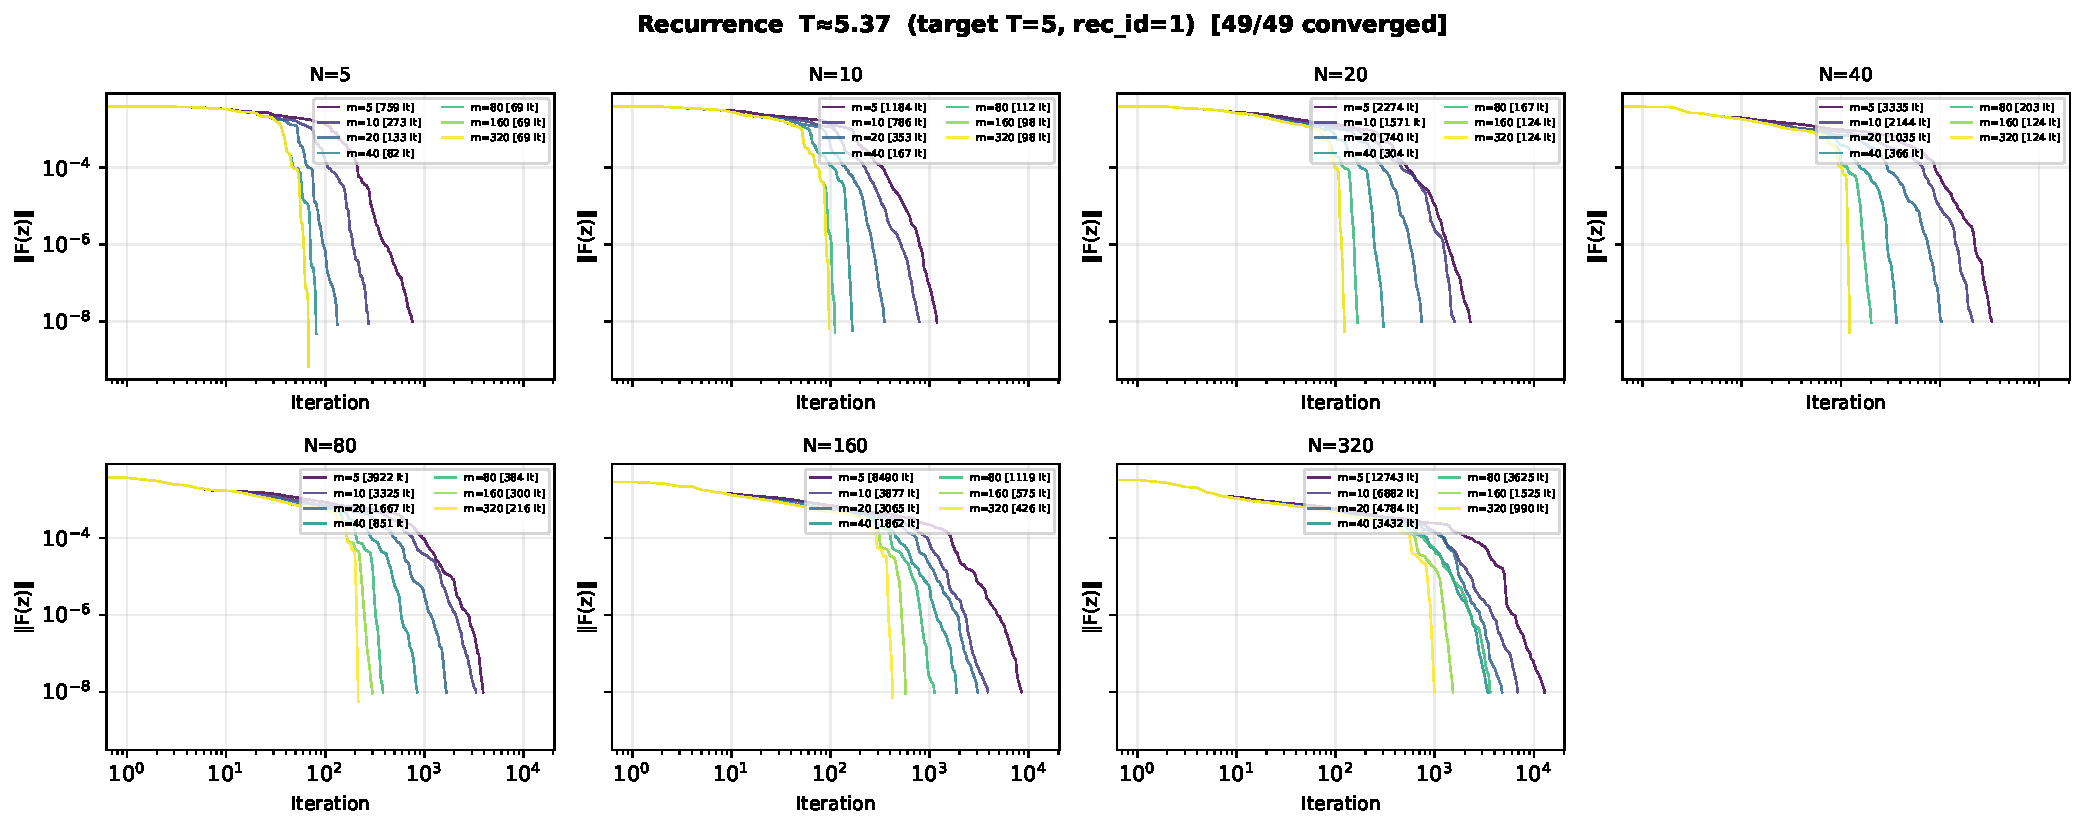
\includegraphics[width=\textwidth]{../analysis/plots/fig01_convergence_curves/fig01_T5_rec001.pdf}
  \caption{Convergence curves for recurrence $T=5$, rec\_id=1.
           Subplots show $\|F(z)\|$ vs.\ iteration for
           each $N$; curves within a subplot correspond to different $m$
           values.  All 49 $(N,m)$ combinations converged for this
           recurrence.}
  \label{fig:convcurves}
\end{figure}

\subsection{Iterations Heatmap (Fig.~6)}
For each recurrence, a $7 \times 7$ heatmap of the $(N,m)$ grid displays the
number of iterations required for convergence (logarithmic colour scale).
Converged cells are annotated with the iteration count; non-converged cells
display a status symbol ($\times$ for incomplete/crashed, $\times_d$ for
diverged, $\times_m$ for hit\_maxiter, $\cdot$ for no\_data).
Figures~\ref{fig:heatmap_T05} and \ref{fig:heatmap_T80} contrast a
short-period recurrence (all 49 combos converged) with a long-period one
(many no\_data/incomplete cells due to the SLURM time limit).

\begin{figure}[H]
  \centering
  \begin{subfigure}{0.48\textwidth}
    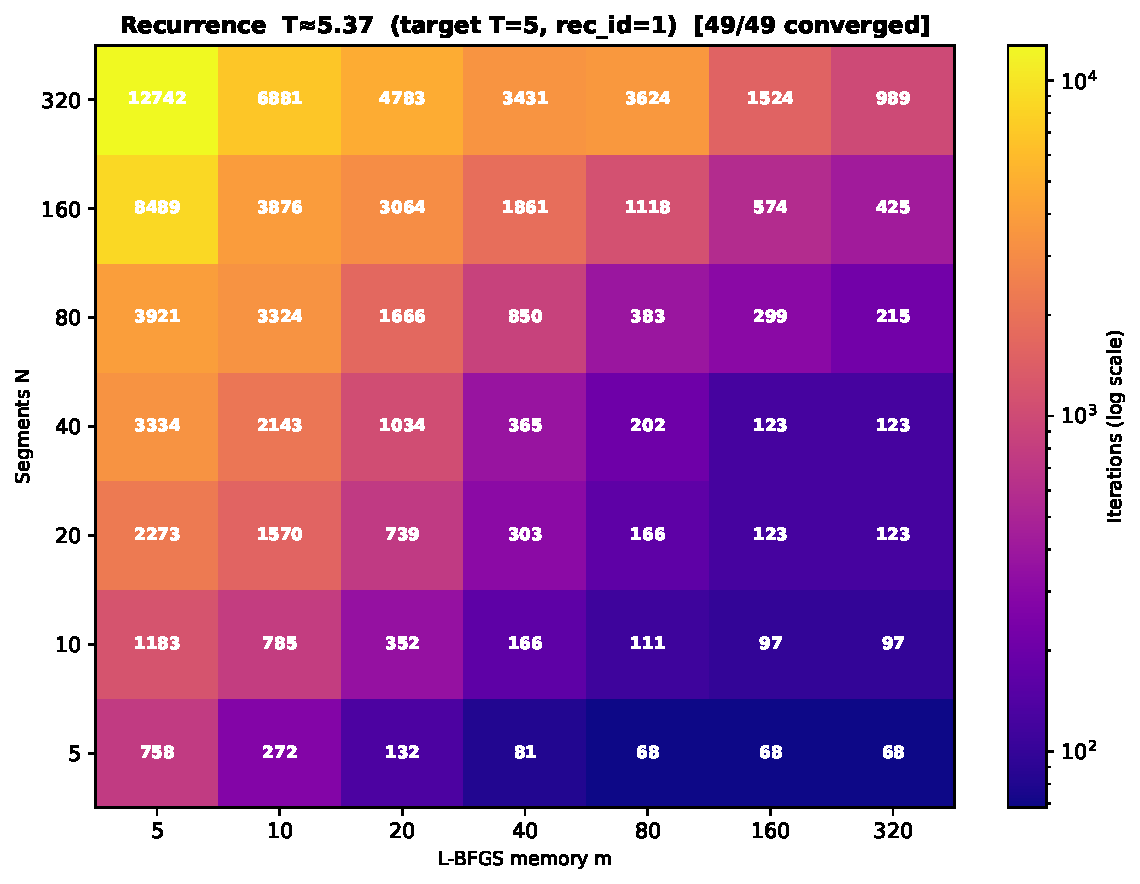
\includegraphics[width=\textwidth]{../analysis/plots/fig06_iterations_heatmap/fig06_T5_rec001.pdf}
    \caption{$T=5$, rec\_id=1.  All 49 combos converged.}
    \label{fig:heatmap_T05}
  \end{subfigure}
  \hfill
  \begin{subfigure}{0.48\textwidth}
    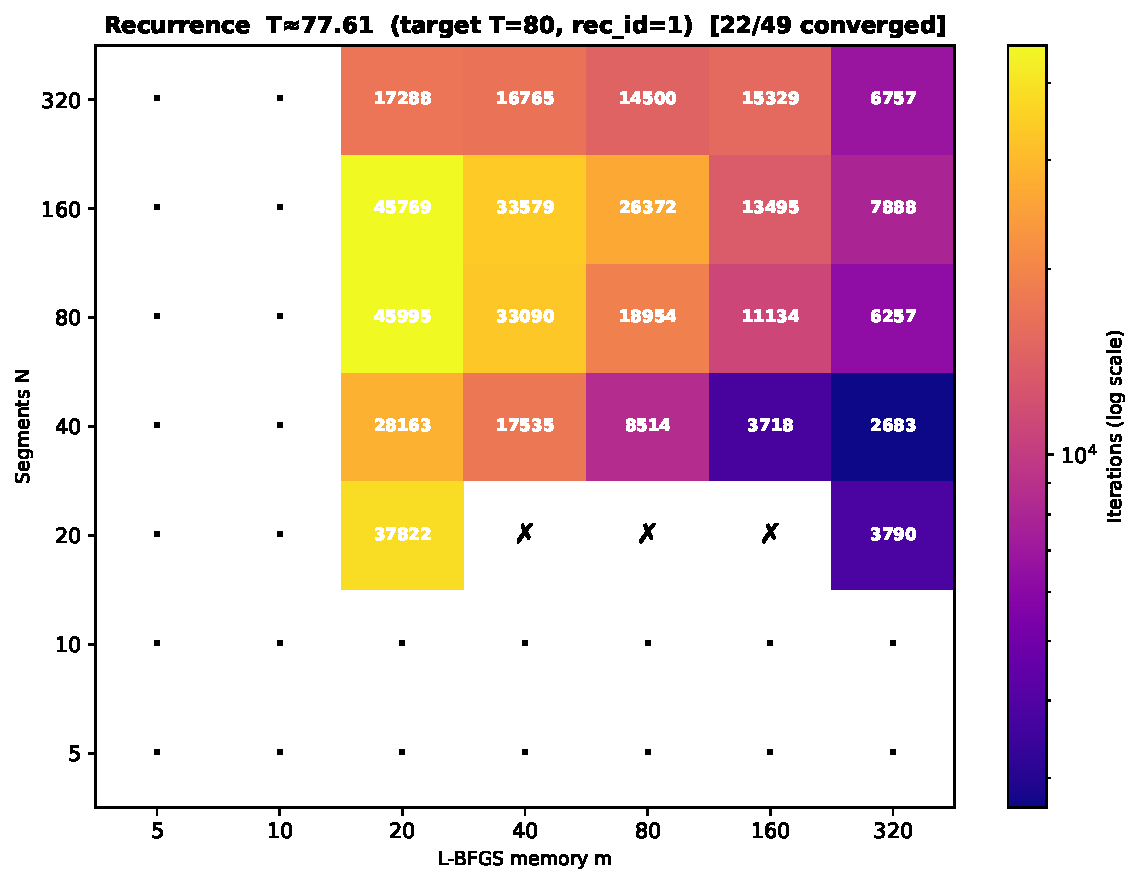
\includegraphics[width=\textwidth]{../analysis/plots/fig06_iterations_heatmap/fig06_T80_rec001.pdf}
    \caption{$T=80$, rec\_id=1.  Many combos did not finish.}
    \label{fig:heatmap_T80}
  \end{subfigure}
  \caption{Per-recurrence iteration heatmaps for two contrasting cases.}
  \label{fig:heatmaps}
\end{figure}

\subsection{Aggregate Bar Charts}
Four aggregate plots summarise the full dataset across all recurrences,
ordered by actual converged period $T$.

\begin{figure}[H]
  \centering
  
\includegraphics[width=\textwidth]{../analysis/plots/convcount_vs_T.pdf}
  \caption{Convergence count per recurrence (out of 49 max).  Most
           short-period recurrences achieve the maximum 49/49, while
           long-period recurrences show a broader spread.}
  \label{fig:convcount}
\end{figure}

\begin{figure}[H]
  \centering
  
\includegraphics[width=\textwidth]{../analysis/plots/maxiter_vs_T.pdf}
  \caption{Iterations of the slowest converged $(N,m)$ combination for each
           recurrence.  This indicates the worst-case computational cost for
           a given orbit.}
  \label{fig:maxiter}
\end{figure}

\begin{figure}[H]
  \centering
  
\includegraphics[width=\textwidth]{../analysis/plots/best3_combos_vs_T.pdf}
  \caption{Slowest converged combo per recurrence (grey bars), with the
           three fastest $(N,m)$ combinations overlaid as coloured scatter
           markers.  This reveals whether the fastest combinations cluster
           around particular parameter values.}
  \label{fig:best3}
\end{figure}

\begin{figure}[H]
  \centering
  
\includegraphics[width=\textwidth]{../analysis/plots/fastest_bar_annotated.pdf}
  \caption{Fastest converged $(N,m)$ combination per recurrence.  Each bar
           is annotated with the recurrence ID, actual converged period $T$,
           and the winning $(N,m)$ pair.}
  \label{fig:fastest}
\end{figure}

\subsection{Aggregate Heatmaps per Period}
To summarise convergence behaviour across all recurrences for a given target
period, we produce a two-panel figure for each $T$: the left panel shows the
median number of L-BFGS iterations to convergence for each $(N,m)$ pair
(logarithmic colour scale), and the right panel shows the fraction of
recurrences that converged for that pair (green = high success rate, red =
low).  Figures~\ref{fig:agg_T05}--\ref{fig:agg_T160} present the six
aggregate heatmaps.

\begin{figure}[H]
  \centering
  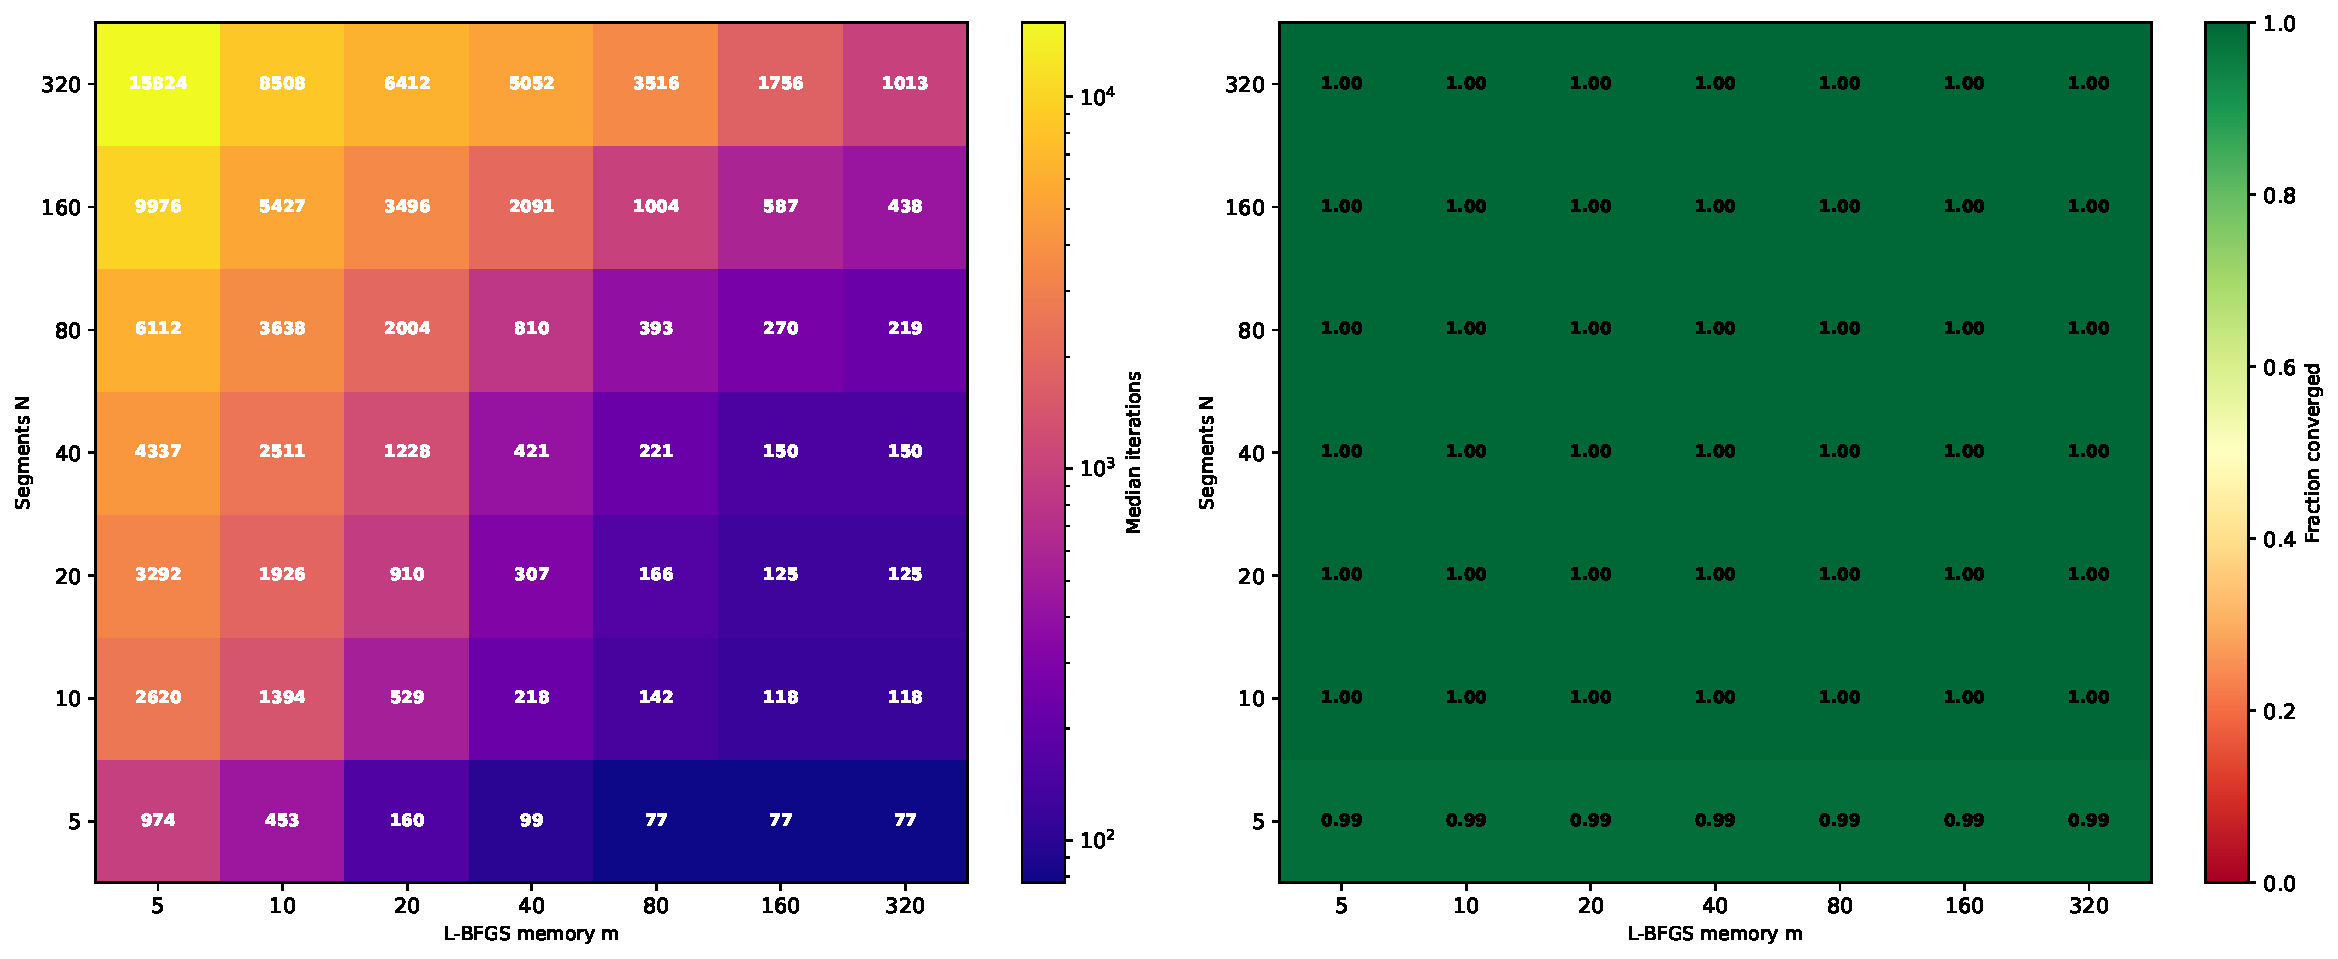
\includegraphics[width=\textwidth]{../analysis/plots/agg_heatmaps/agg_heatmap_T05.pdf}
  \caption{Aggregate heatmap for $T=5$: median iterations (left) and
           convergence success rate (right) across all 84 recurrences.}
  \label{fig:agg_T05}
\end{figure}

\begin{figure}[H]
  \centering
  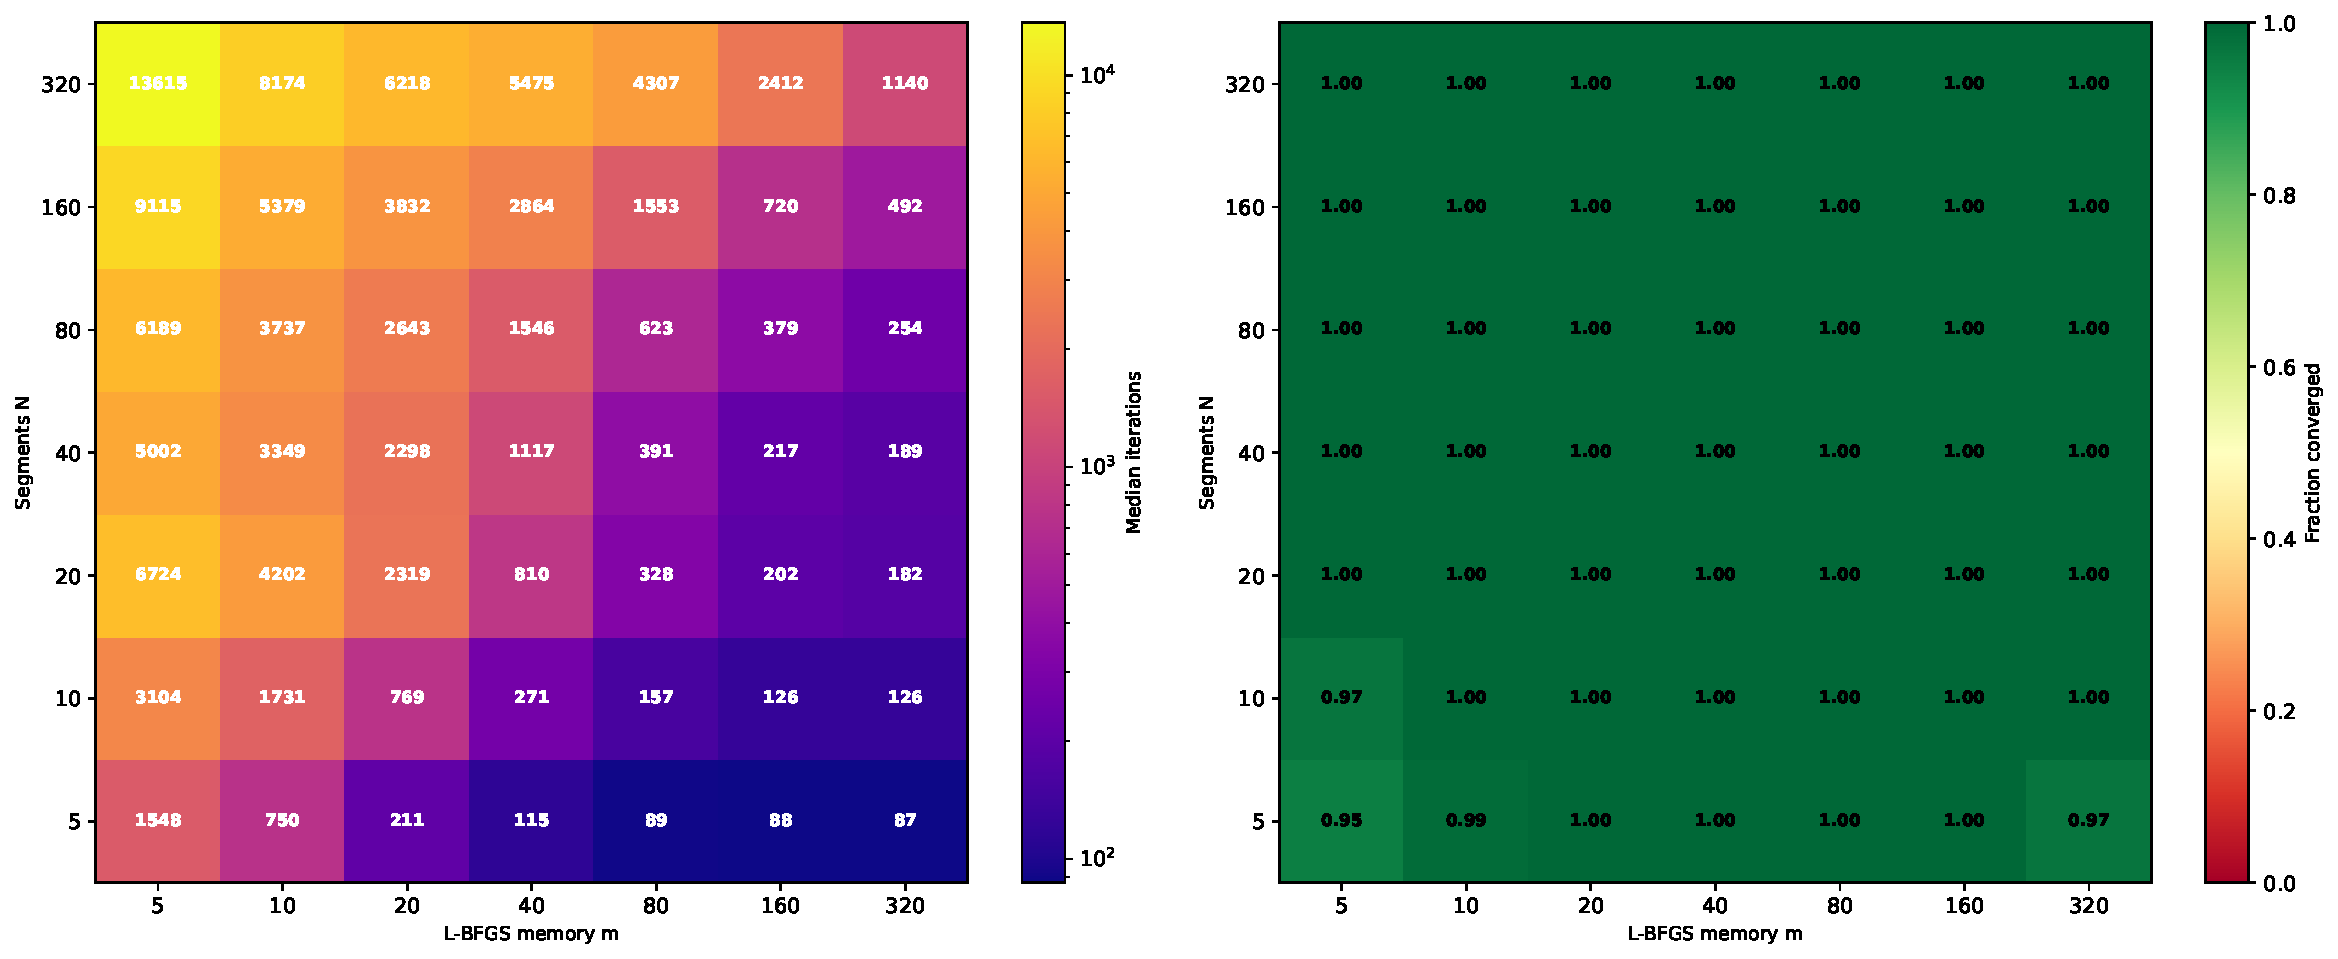
\includegraphics[width=\textwidth]{../analysis/plots/agg_heatmaps/agg_heatmap_T10.pdf}
  \caption{Aggregate heatmap for $T=10$ (99 recurrences).}
  \label{fig:agg_T10}
\end{figure}

\begin{figure}[H]
  \centering
  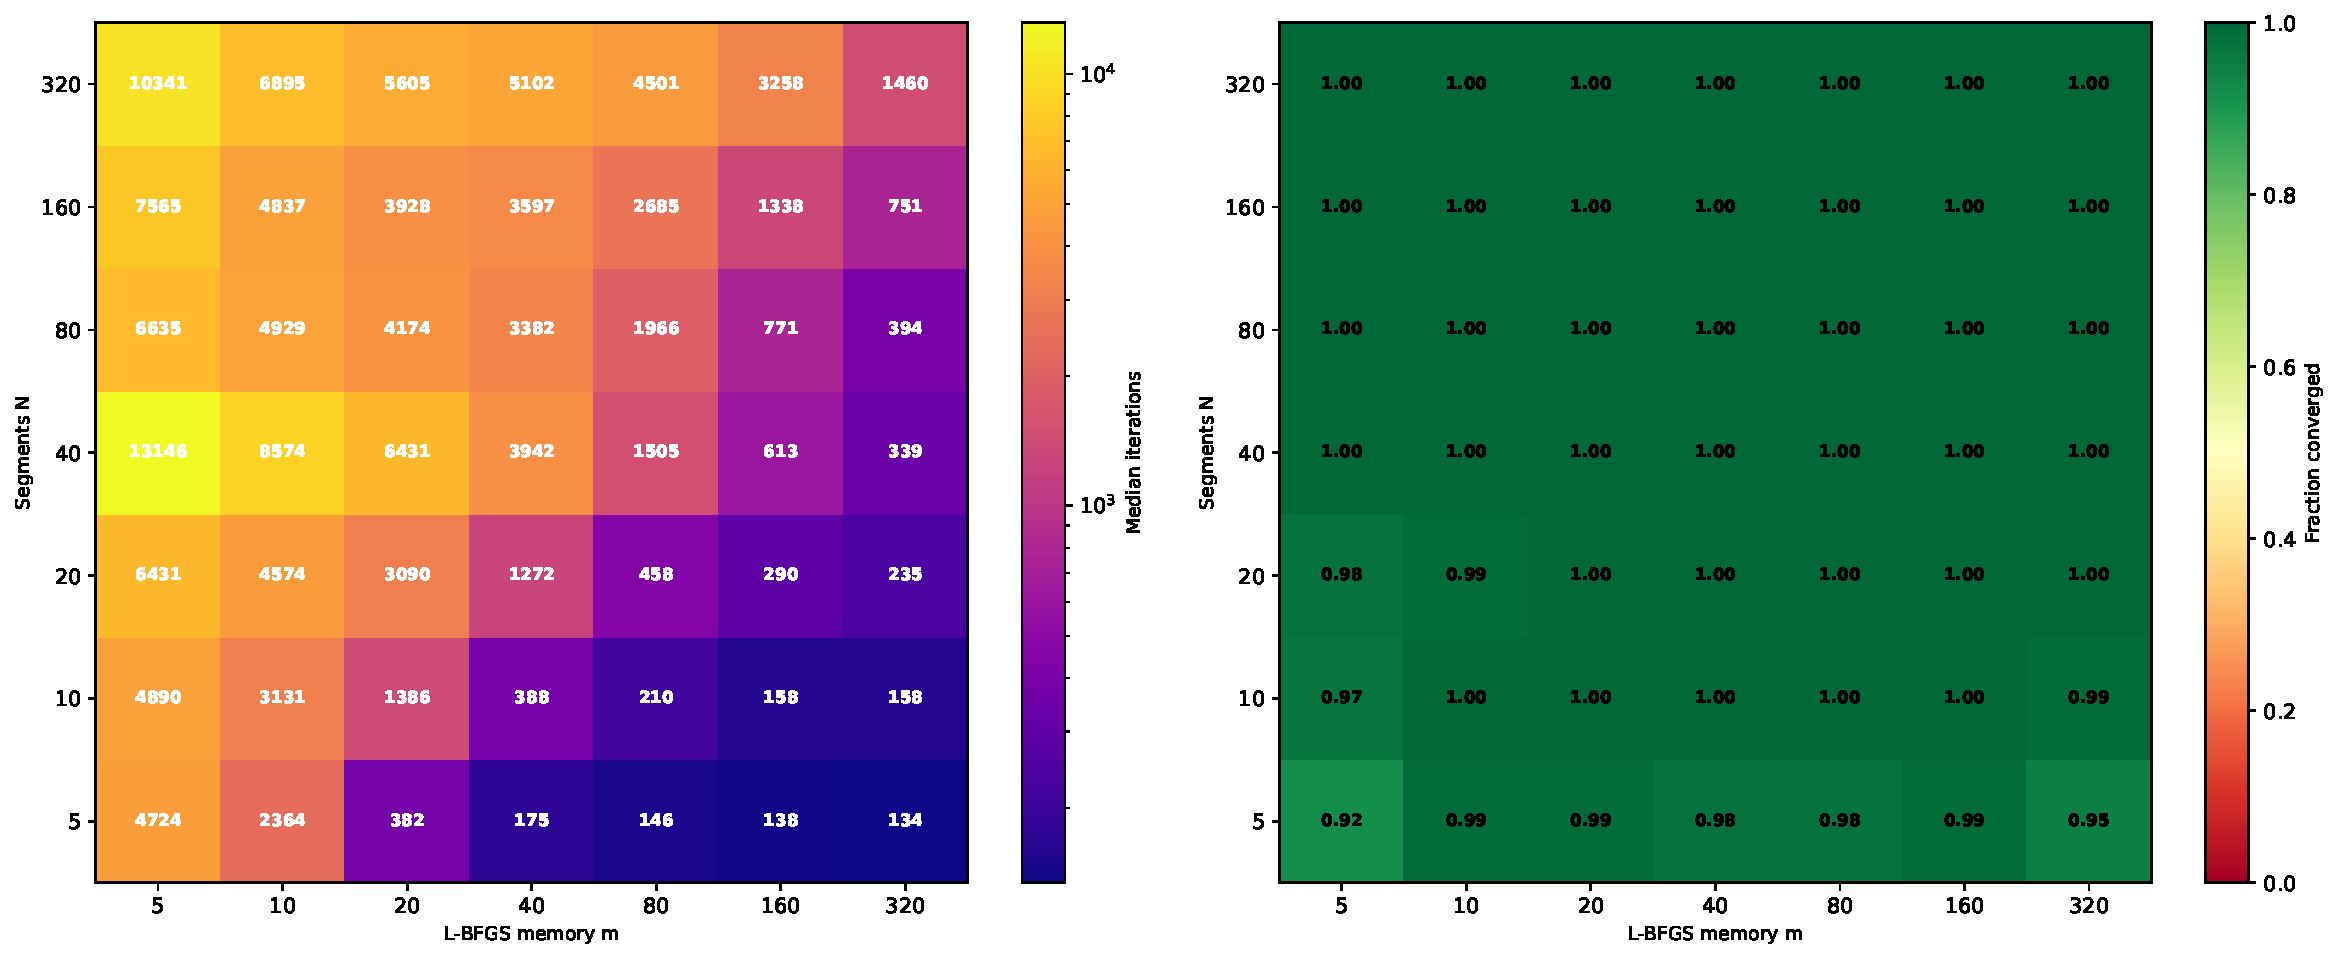
\includegraphics[width=\textwidth]{../analysis/plots/agg_heatmaps/agg_heatmap_T20.pdf}
  \caption{Aggregate heatmap for $T=20$ (99 recurrences).  The optimal $N$
           remains at 5, but $m=320$ begins to overtake $m=160$.}
  \label{fig:agg_T20}
\end{figure}

\begin{figure}[H]
  \centering
  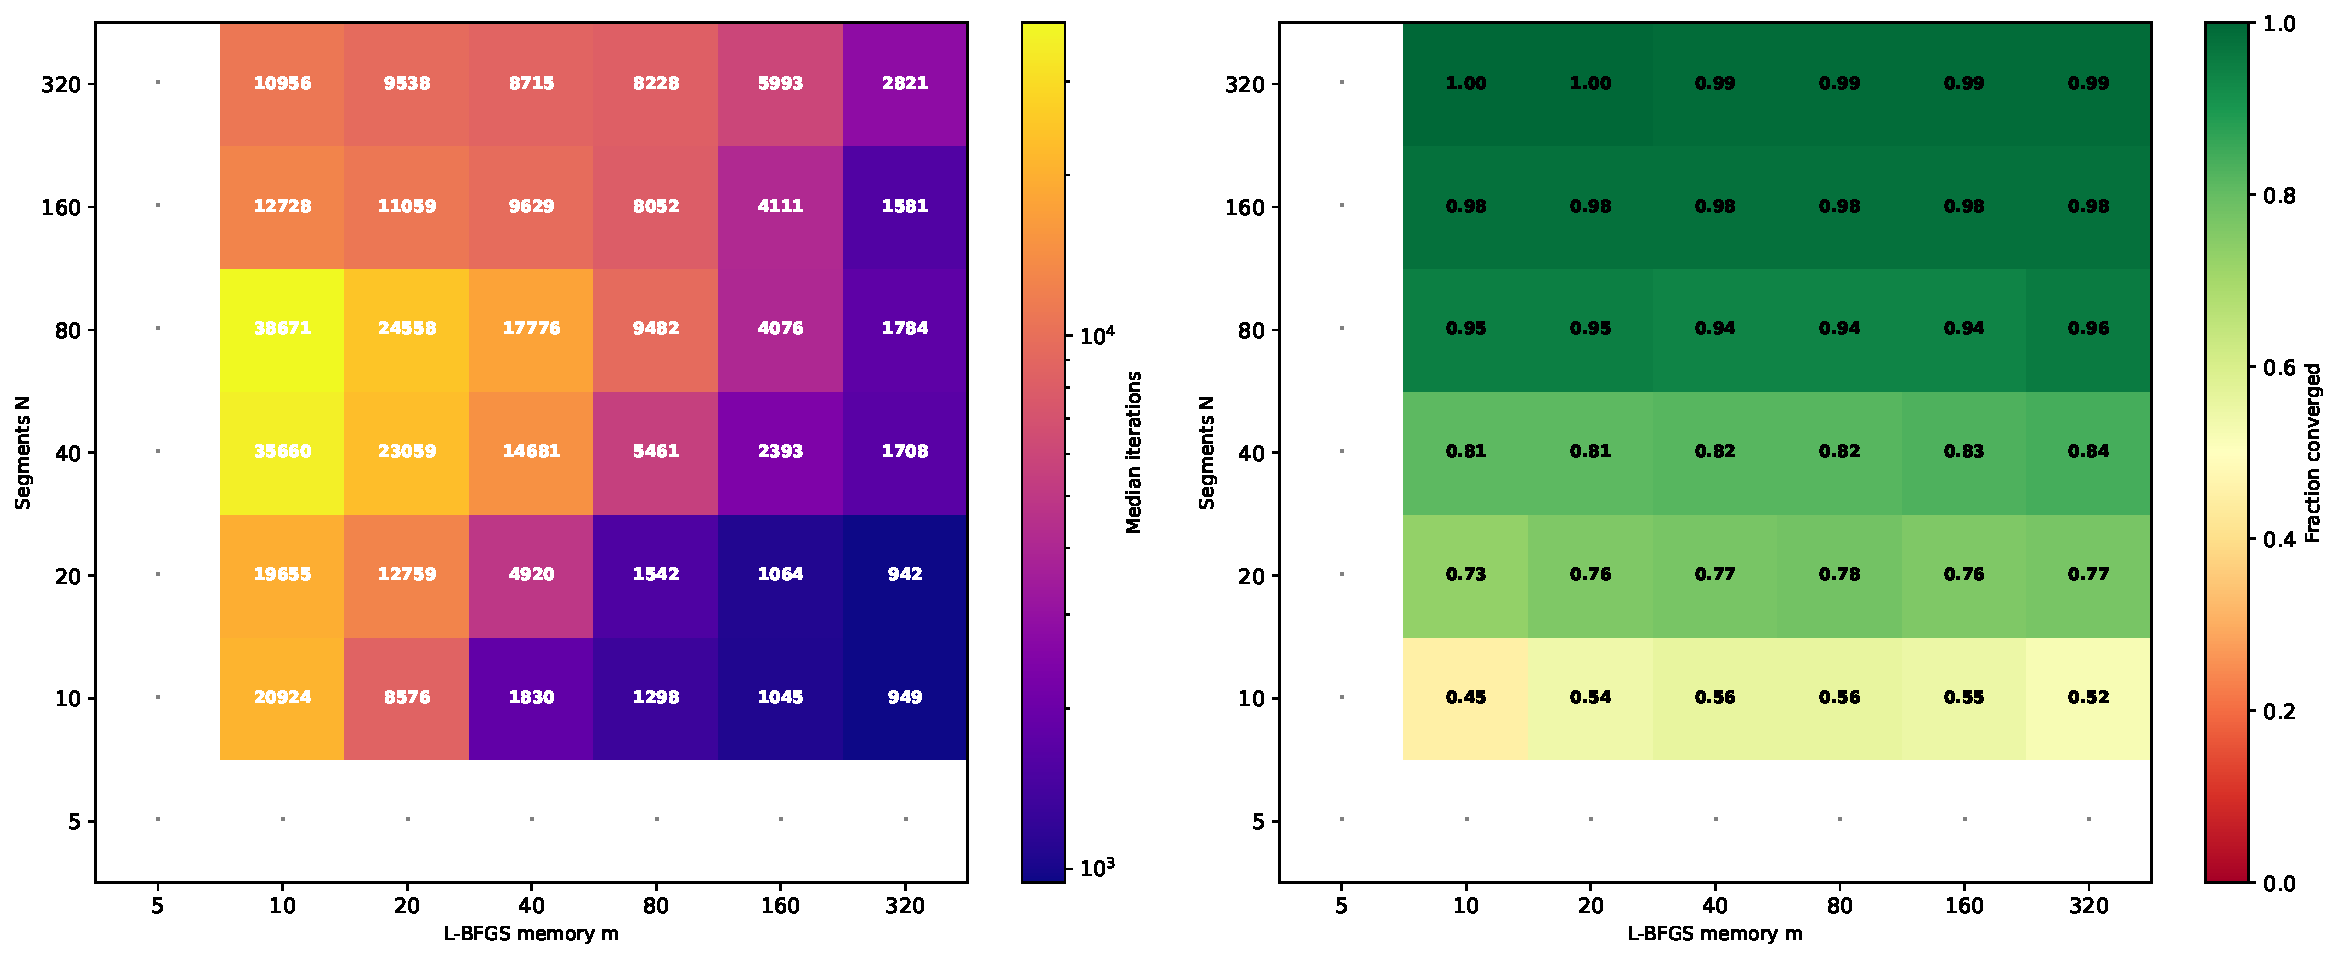
\includegraphics[width=\textwidth]{../analysis/plots/agg_heatmaps/agg_heatmap_T40.pdf}
  \caption{Aggregate heatmap for $T=40$ (100 recurrences).  The optimal $N$
           shifts to 20; small $N$ and $m$ values (excluded \textit{a
           priori}) appear blank.}
  \label{fig:agg_T40}
\end{figure}

\begin{figure}[H]
  \centering
  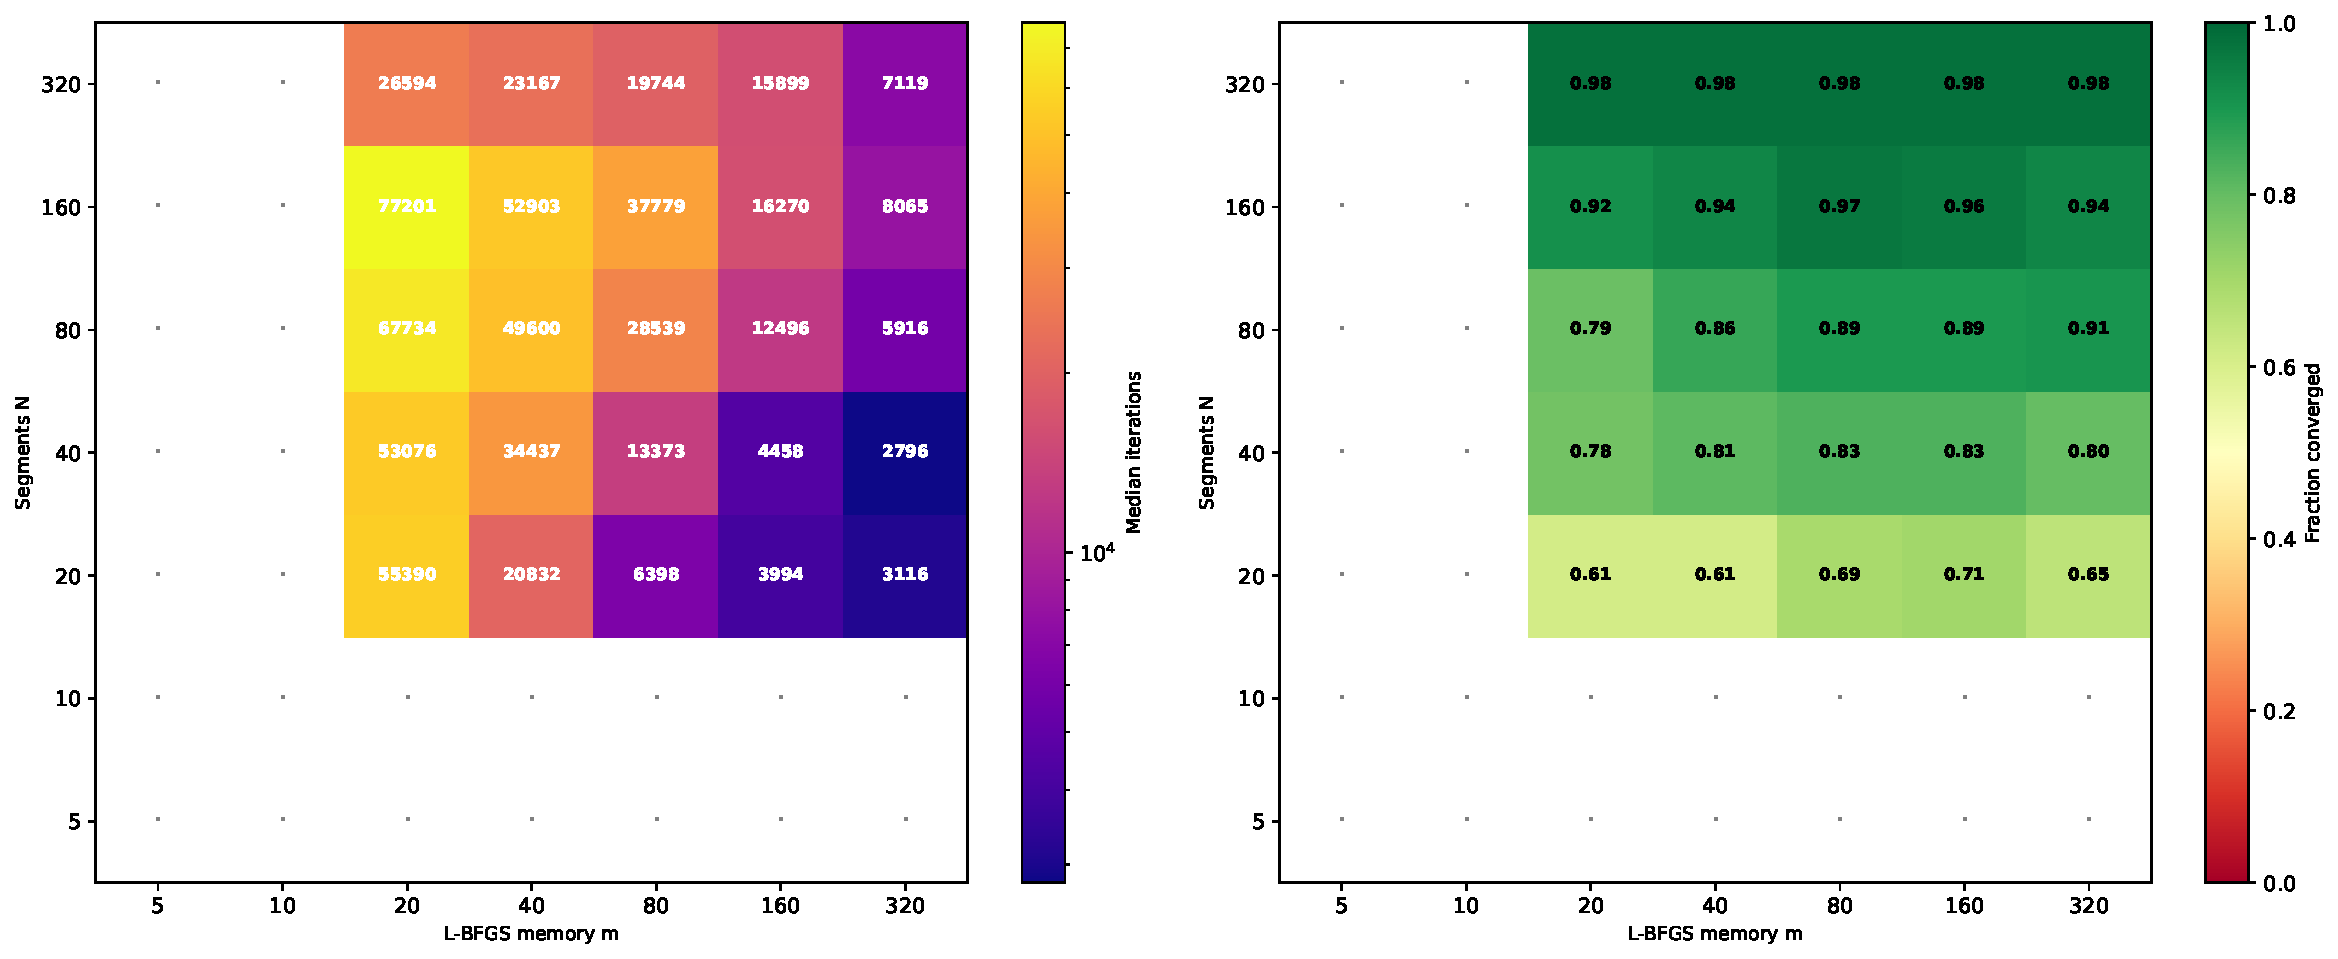
\includegraphics[width=\textwidth]{../analysis/plots/agg_heatmaps/agg_heatmap_T80.pdf}
  \caption{Aggregate heatmap for $T=80$ (95 recurrences).  Optimal $N$
           shifts to 40; $m=320$ dominates the high-success region.}
  \label{fig:agg_T80}
\end{figure}

\begin{figure}[H]
  \centering
  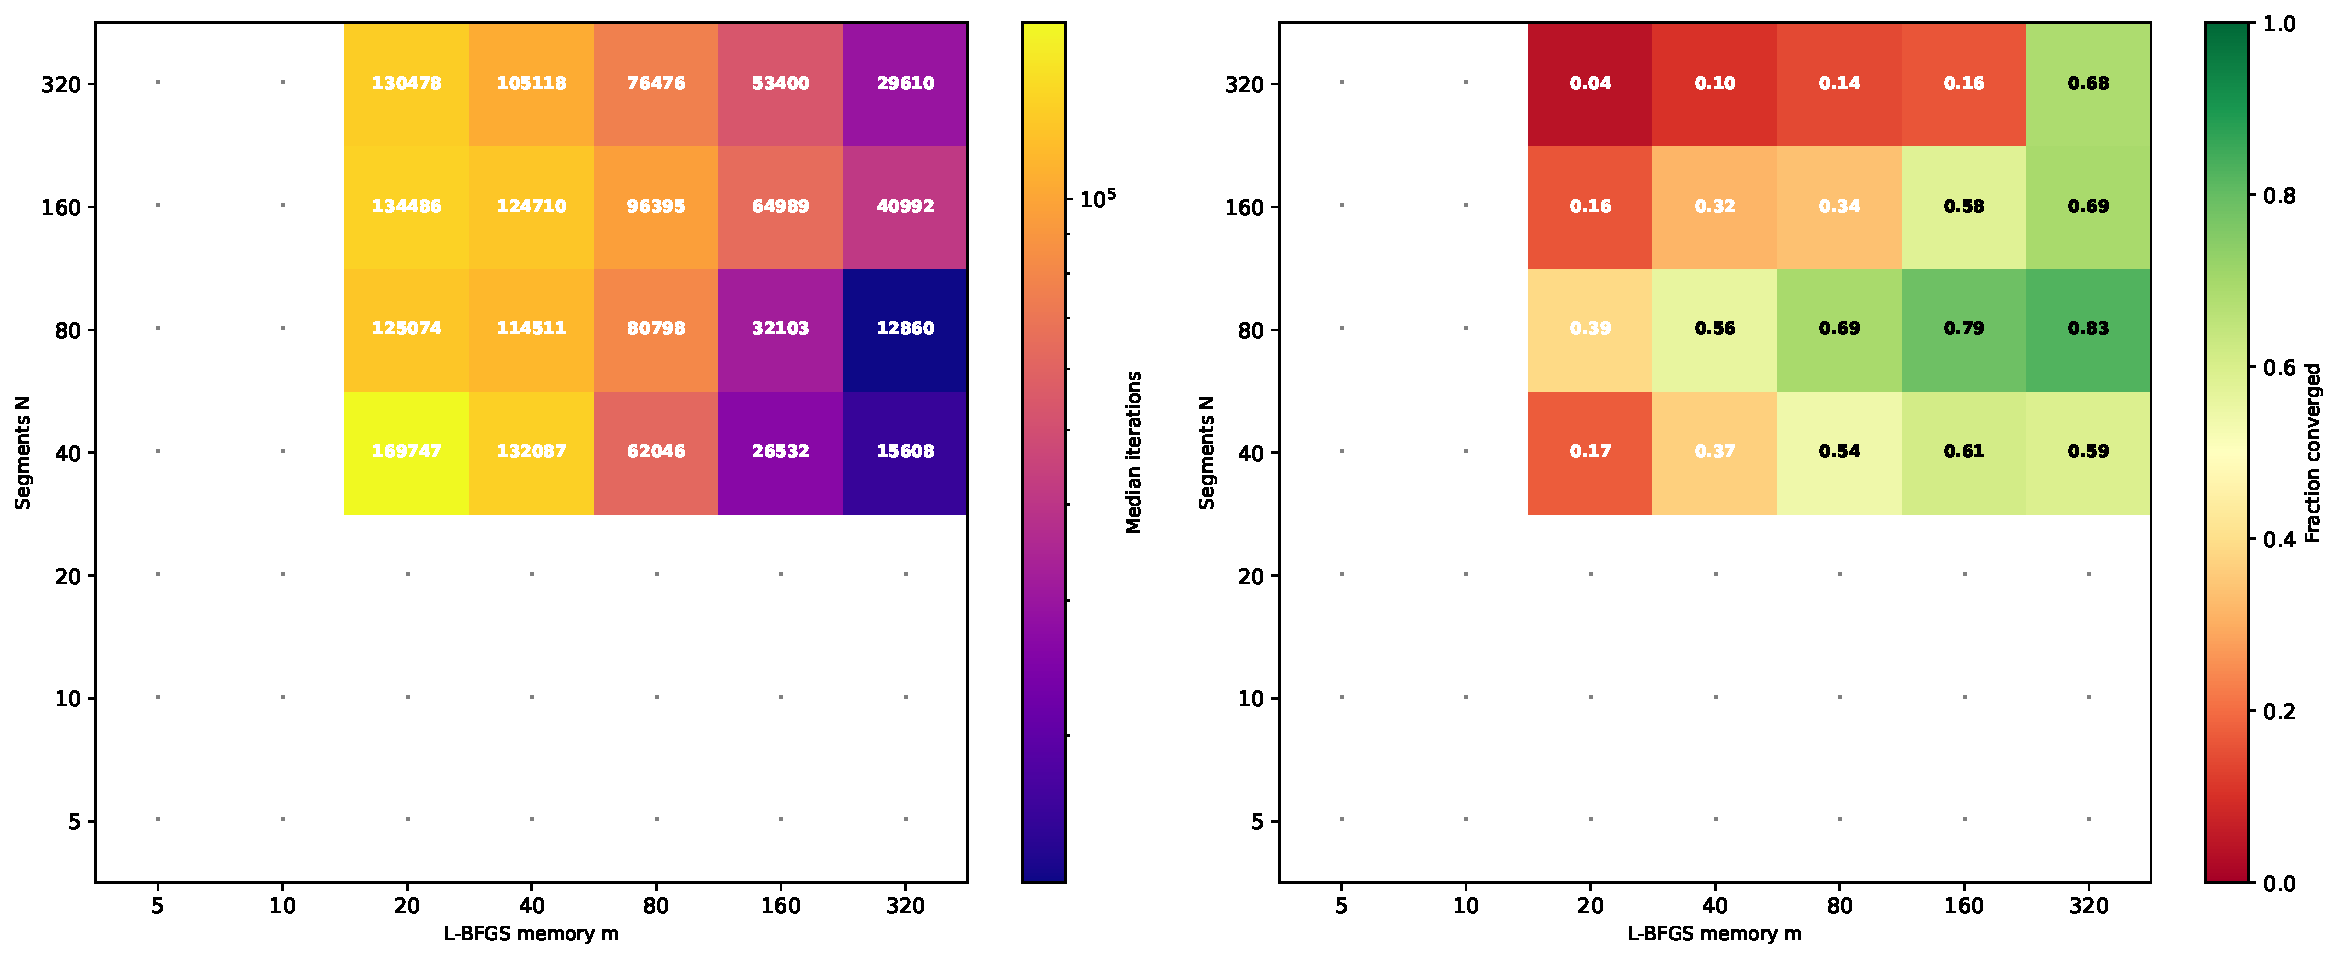
\includegraphics[width=\textwidth]{../analysis/plots/agg_heatmaps/agg_heatmap_T160.pdf}
  \caption{Aggregate heatmap for $T=160$ (98 recurrences).  Optimal $N=80$;
           the convergence rate drops substantially, reflecting the intrinsic
           difficulty of long-period orbits.}
  \label{fig:agg_T160}
\end{figure}

% ============================================================================
\section{Best Parameter Pairs per Period}
% ============================================================================

A key practical question is: \emph{which $(N,m)$ combination is most likely
to converge fastest for a given target period?}  To answer this, we tabulate,
for each $T$, the $(N,m)$ pair that delivers the fewest iterations on the
largest number of recurrences (the ``winner''), together with the
runner-up.  Table~\ref{tab:best_pairs} presents these results.

\begin{table}[htbp]
  \centering
  \caption{Best $(N,m)$ pair per target period.  ``Wins'' counts how many
           recurrences (out of those with at least one converged combo) are
           converged fastest by the given pair.  The win fraction is
           wins / total\_recs\_with\_converged.}
  \label{tab:best_pairs}
  \begin{tabular}{@{}lrrrrrrr@{}}
    \toprule
    \textbf{T} & \textbf{Best} $N$ & \textbf{Best} $m$ & \textbf{Wins} &
    \textbf{Total} & \textbf{Fraction} &
    \textbf{Runner-up} $N$ & \textbf{Runner-up} $m$ \\
    \midrule
    5   & 5   & 160 & 73  & 84  & 86.9\% & 5   & 80  \\
    10  & 5   & 160 & 82  & 99  & 82.8\% & 5   & 320 \\
    20  & 5   & 320 & 68  & 99  & 68.7\% & 5   & 160 \\
    40  & 20  & 320 & 35  & 100 & 35.0\% & 160 & 320 \\
    80  & 40  & 320 & 46  & 95  & 48.4\% & 20  & 320 \\
    160 & 80  & 320 & 49  & 98  & 50.0\% & 40  & 320 \\
    \bottomrule
  \end{tabular}
\end{table}

Several clear trends emerge from Table~\ref{tab:best_pairs}:

\begin{enumerate}[label=(\roman*)]
  \item \textbf{Short periods favour few segments.}  For $T \le 20$, the
        optimal number of shooting segments is $N = 5$ --- the smallest value
        in the sweep.  This is remarkable: a single near-recurrence, seeded
        with just 5 shooting points, converges robustly to a periodic orbit
        for over 99\% of candidates.  The exponential amplification over
        $T/N \le 4$ time units is evidently manageable for the Lorenz
        attractor at these periods.

  \item \textbf{Optimal $N$ scales with $T$.}  As the period increases,
        the best $N$ grows from 5 ($T=5$) to 80 ($T=160$), keeping the
        segment duration $T/N$ in the range $1$--$2$ time units.  This is
        consistent with the multiple-shooting motivation: the segment
        integration time must be kept below the Lyapunov time
        $1/\lambda \approx 1.1$ for the Jacobian to remain well-conditioned.

  \item \textbf{Large L-BFGS memory is universally beneficial.}
        $m = 320$ (the maximum value in the sweep) is either the best or the
        runner-up memory size for \emph{every} target period.  This suggests
        that the Hessian approximation benefits from retaining as much
        curvature history as possible, and that the storage cost of $m=320$
        pairs ($\sim\!320 \times 961$ floating-point numbers $\approx 2.5$
        MB) is negligible relative to the computational cost of the
        line-search and flow integrations.

  \item \textbf{Win fractions decrease with $T$.}  For $T=5$, a single
        $(N,m)=(5,160)$ pair is fastest for 87\% of recurrences.  For
        $T=160$, the best pair $(80,320)$ wins only 50\% of the time.  This
        indicates that long-period orbits are more heterogeneous: different
        orbits benefit from different $(N,m)$ combinations, and no single
        choice dominates.
\end{enumerate}

% ============================================================================
\section{Summary and Discussion}
% ============================================================================

We have presented a complete computational pipeline for discovering periodic
orbits of the Lorenz system.  The approach combines (i)~a streaming
distance-matrix method to detect near-recurrence candidates from a long
trajectory, (ii)~a multiple-shooting formulation that renders the
root-finding problem well-conditioned, (iii)~L-BFGS optimisation to refine
each candidate to machine precision, and (iv)~an embarrassingly parallel HPC
deployment that scales to $\sim$29,000 independent cases on the Iridis~X
cluster.

The key findings are:

\begin{itemize}
  \item Near-recurrence detection with a $\pm 20\%$ period tolerance and
        spatial deduplication ($\delta_{\min} = 3.0$) reliably produces
        $\sim$100 distinct candidates per target period.

  \item Short-period orbits ($T \le 20$) converge with $>\!99\%$ success
        rate using as few as $N = 5$ shooting segments, demonstrating the
        quality of the near-recurrence initial guesses.

  \item For longer periods, the optimal number of segments scales as
        $N \propto T$, keeping the per-segment integration time below the
        Lyapunov time.  The largest L-BFGS memory ($m = 320$) is
        consistently the best or near-best choice.
\end{itemize}

The complete dataset --- including per-iteration histories, converged
trajectories, classification tables, and diagnostic plots --- is available
in the project repository.  The pipeline is modular and can be adapted to
other dynamical systems by replacing the Lorenz-specific flow and
linearisation operators.

% ============================================================================
\section{Outlook and Future Work}
% ============================================================================

The present work demonstrates a robust, scalable pipeline for computing
periodic orbits of the Lorenz system.  Several natural extensions present
themselves.

\subsection{Application to Other Fluid-Dynamical Systems}
The pipeline is modular: the recurrence finder, the multiple-shooting
formulation, and the L-BFGS optimiser are agnostic to the specific dynamical
system.  Only the flow operators $\varphi$, $\Phi$, and $\Psi$ need to be
replaced.  A natural next target is the \textbf{Open Kolmogorov Flow}
(OKF)~\cite{chandler2022open}, a two-dimensional, doubly-periodic,
spatially-extended Navier--Stokes configuration that exhibits a rich
hierarchy of exact coherent structures including travelling waves, periodic
orbits, and relative periodic orbits.

\subsection{Computational-Time Callbacks and Algorithm Comparison}
A natural question is how L-BFGS compares with other solvers available in
NKSearch.jl, particularly the \textbf{Newton--GMRES Hookstep}
(trust-region) method~\cite{sanchez2004newton}.  The hookstep method solves
$J(z)\,\delta z = -F(z)$ matrix-free at each Newton iteration: GMRES
approximately solves the linear system, and the step is constrained to lie
within a trust region of radius $\Delta$.  Unlike L-BFGS, the hookstep
method does not require adjoint integration (only the forward linearised
flow $\Phi$), making each iteration computationally cheaper.  However, it
typically requires more iterations to converge because the trust-region
constraint limits the step size, and the GMRES tolerance must be carefully
balanced against the outer Newton tolerance.

To compare these methods fairly, one needs a \textbf{computational-time
callback} in NKSearch.jl that records the elapsed CPU (or wall-clock) time
at each iteration alongside the residual norm.  Such a callback is
orthogonal to the existing per-iteration logging --- it adds a time-stamp
column to the CSV output, enabling plots of $\|F(z)\|$ versus
\textit{compute time} rather than iteration count.  This would allow
questions such as ``which method reaches $\|F\| = 10^{-8}$ in the shortest
wall-clock time?'' to be answered quantitatively.  A preliminary comparison
on the Open Kolmogorov Flow system would be particularly instructive, since
the higher state-space dimension of OKF (hundreds to thousands of degrees of
freedom, versus three for Lorenz) amplifies the cost difference between
adjoint-based and adjoint-free methods.  The callback would also record the
time spent in each computational phase (residual evaluation, gradient
computation, GMRES iterations, line search), yielding a detailed performance
profile.

% ============================================================================
% Bibliography
% ============================================================================
\begin{thebibliography}{9}

\bibitem{lorenz1963deterministic}
E.~N.~Lorenz.
\newblock Deterministic nonperiodic flow.
\newblock \emph{Journal of the Atmospheric Sciences}, 20(2):130--141, 1963.

\bibitem{cvitanovic2016chaos}
P.~Cvitanovi\'{c}, R.~Artuso, R.~Mainieri, G.~Tanner, and G.~Vattay.
\newblock \emph{Chaos: Classical and Quantum}.
\newblock Niels Bohr Institute, Copenhagen, 2012.
\newblock \url{http://chaosbook.org/}

\bibitem{nocedal2006numerical}
J.~Nocedal and S.~J.~Wright.
\newblock \emph{Numerical Optimization}, 2nd ed.
\newblock Springer, New York, 2006.

\bibitem{sanchez2004newton}
J.~S\'{a}nchez, M.~Net, B.~Garc\'{i}a-Archilla, and C.~Sim\'{o}.
\newblock Newton--Krylov continuation of periodic orbits for Navier--Stokes
         flows.
\newblock \emph{Journal of Computational Physics}, 201(1):13--33, 2004.

\bibitem{chandler2022open}
G.~J.~Chandler and R.~R.~Kerswell.
\newblock Invariant recurrent solutions embedded in a turbulent
         two-dimensional Kolmogorov flow.
\newblock \emph{Journal of Fluid Mechanics}, 722:554--595, 2013.

\bibitem{liu1989limited}
D.~C.~Liu and J.~Nocedal.
\newblock On the limited memory BFGS method for large scale optimization.
\newblock \emph{Mathematical Programming}, 45(1--3):503--528, 1989.

\end{thebibliography}

\end{document}
